%-----------------------------------------------------------------------------
%
%               Template for sigplanconf LaTeX Class
%
% Name:         sigplanconf-template.tex
%
% Purpose:      A template for sigplanconf.cls, which is a LaTeX 2e class
%               file for SIGPLAN conference proceedings.
%
% Guide:        Refer to "Author's Guide to the ACM SIGPLAN Class,"
%               sigplanconf-guide.pdf
%
% Author:       Paul C. Anagnostopoulos
%               Windfall Software
%               978 371-2316
%               paul@windfall.com
%
% Created:      15 February 2005
%
%-----------------------------------------------------------------------------


\documentclass{sigplanconf}

% The following \documentclass options may be useful:

% preprint      Remove this option only once the paper is in final form.
% 10pt          To set in 10-point type instead of 9-point.
% 11pt          To set in 11-point type instead of 9-point.
% authoryear    To obtain author/year citation style instead of numeric.
\usepackage{epsfig,endnotes}
\usepackage{graphicx}
\usepackage{epstopdf}
\usepackage{setspace}
\usepackage{algpseudocode}
\usepackage{multirow}
%\usepackage{subfigure}
\usepackage[ruled,lined]{algorithm2e}
\usepackage{wrapfig, floatflt}
%\usepackage{subfig}
\usepackage{subfigure}

\usepackage{amsmath}

%------------------------------------------------------------------------------
%                  Useful commands and acronymns used in the paper.
%------------------------------------------------------------------------------
% Commands
\newcommand{\mycomment}[1]{}
\newcommand{\ignore}[1]{}
%\ifpdf
%\renewcommand{\url}[1]{\texttt{\small{#1}}}
%\else
%\newcommand{\url}[1]{\texttt{\small{#1}}}
%\fi
\newcommand{\code}[1]{\texttt{#1}}
\newcommand{\codesm}[1]{\texttt{\small #1}}
\newcommand{\sm}[1]{{\small #1}}
\newcommand{\mycaption}[2]{\textbf{\textsf{\caption{#1}#2}}}

\newcommand{\todo}[1]{\textbf{TODO [#1]???}} 
\newcommand{\fixme}[1]{\textbf{FIXME [#1]???}} 
\newcommand{\remark}[1]{\textbf{REMARK [#1]???}} 

% Acronymns
\newcommand{\apriori}{\textit{a priori}}
\newcommand{\adhoc}{ad hoc}
\newcommand{\etal}{\textit{et al.}}
\newcommand{\eg}{\textit{e.g.}}
\newcommand{\ie}{\textit{i.e.}}
\newcommand{\mybull}{\noindent $\bullet$~}
\newcommand{\ms}{$ms$~}
\newcommand{\us}{${\mu}s$~}

%\newcommand{\mybull}{}
\newcommand{\mystar}{$\bigstar$}


% Section names, figure names and algorithm names.
\newcommand{\figref}[1]{Figure~\ref{#1}}
\newcommand{\sectref}[1]{Section~\ref{#1}}
\newcommand{\sectrefs}[2]{Sections~\ref{#1}-\ref{#2}}
\newcommand{\aref}[1]{Algorithm~\ref{#1}}
\newcommand{\sect}[1]{\section{#1}}
\newcommand{\subsect}[1]{\subsection{#1}}
\newcommand{\subsubsect}[1]{\subsubsection{#1}}
\newcommand{\mysect}[1]{\subsect{#1}}


\newtheorem{ourtask}{Task}

\begin{document}

\special{papersize=8.5in,11in}
\setlength{\pdfpageheight}{\paperheight}
\setlength{\pdfpagewidth}{\paperwidth}

\conferenceinfo{CONF 'yy}{Month d--d, 20yy, City, ST, Country}
\copyrightyear{20yy}
\copyrightdata{978-1-nnnn-nnnn-n/yy/mm}
\doi{nnnnnnn.nnnnnnn}

% Uncomment one of the following two, if you are not going for the
% traditional copyright transfer agreement.

%\exclusivelicense                % ACM gets exclusive license to publish,
                                  % you retain copyright

%\permissiontopublish             % ACM gets nonexclusive license to publish
                                  % (paid open-access papers,
                                  % short abstracts)

\titlebanner{banner above paper title}        % These are ignored unless
\preprintfooter{short description of paper}   % 'preprint' option specified.

\title{iWarp: Cache Interference-Aware Warp Scheduling for General Purpose Graphic Processing Units}
%\subtitle{Subtitle Text, if any}

\authorinfo{Shuwen Gao}
           {Computer Architecture and Memory Systems Laboratory\\Department of Electrical Engineering\\The University of Texas at Dallas}
           {Shu-wen.Gao@utdallas.edu}
\authorinfo{Myoungsoo Jung}
           {Computer Architecture and Memory Systems Laboratory\\Department of Electrical Engineering\\The University of Texas at Dallas}
           {jung@utdallas.edu}

\maketitle

\begin{abstract}
This is the text of the abstract.
\end{abstract}

\category{CR-number}{subcategory}{third-level}

% general terms are not compulsory anymore,
% you may leave them out
\terms
term1, term2

\keywords
keyword1, keyword2

\section{Introduction}

The text of the paper begins here.


\section{Background}
In this section, we briefly explain the fundamental organization of our baseline GPU device. We then look into the nature of cache contention in a streaming multiprocessor environment, which in turn can introduce a significant performance degradation in diverse data-intensive workloads. Finally, we discuss the three categories of conventional and recently proposed warp scheduling policies that are implemented by the existing GPGPU designs to counter the stifling effect of cache contention.

\subsection{Baseline GPGPU Architecture}

A GPU device in typical consists of multiple \textit{streaming multiprocessors} (SMs), which are also known as \textit{single instruction multiple thread} (SIMT) computational units. Figures \ref{fig:gpu} illustrates our baseline architecture, which essentially resembles NVIDIA's Fermi GPU \cite{nvidia2009nvidia}, and the corresponding micro-architecture of the SM, respectively. Specifically, our baseline GPU employs 15 streaming multiprocessors with 32 CUDA cores and memory partition of 256 byte width. As shown in Figure \ref{fig:gpu}, each memory partition is composed by a shared L2 cache, global DRAM and the corresponding memory controller (MC), and is attached to the interconnect network as off-chip resources. In contrast, a private L1 data cache (L1D), a read-only texture cache, a constant cache, and a shared-memory exist within each SM as on-chip storage resources. Thanks to this scalable and programmable hardware processors, it is significantly easier to map existing data-intensive applications to the massive parallel computation model of a modern GPU device compared to the earlier generations of hardwired pipeline GPUs \cite{lindholm2008nvidia}.
With a state-of-the-art GPU programming interface, such as CUDA \cite{nvidia2008programming} or OpenCL \cite{munshi2009opencl}, an GPU application can comprise of one or more computation \textit{kernels} \cite{nvidia2008programming}, also known as grids \cite{nvidia2008programming}, each of which contains multiple threads. In our baseline architecture, a kernel can contain up to 23,040 lightweight threads. In practice, modern GPUs batch together groups of such individual threads, and execute them on an SM in lock-step fashion with single instruction, multiple data (SIMD) pipeline. Once a target kernel is launched into the GPU device, the lightweight threads are assigned to each SM as clusters of threads termed as \emph{cooperative thread arrays (CTAs)}. These CTAs execute the same kernel program instance but process different chunks of data. The corresponding thread blocks (in a CTA) are synchronized by barriers to communicate with each other through shared and global memory \cite{lindholm2008nvidia}.
The number of CTAs assigned to each SM depends on the on-chip resources available on the SM (i.e., register files, shared memory and barriers that are needed for each CTA).
Within the SM, threads are managed, scheduled and executed in groups of 32, called \emph{warps} \cite{lindholm2008nvidia} (also known as wavefront in AMD GPU \cite{sdk2010v2}).
The multiple threads in warp(s) are managed by a warp scheduler. Such thread groups share the same instruction, but process different data, in parallel. For example, in our baseline, it employs two warp schedulers for each SM. At the issue stage, per cycle, the schedulers select two warps from a list of ready warps to be executed based on a specific scheduling policy that we will explain shortly.

\begin{figure}
\begin{center}
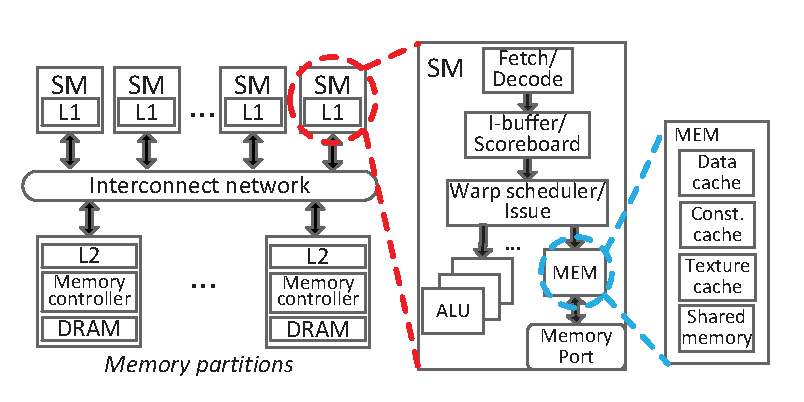
\epsfig{file=figs/gpu.eps,angle=-0,width=0.45\textwidth,clip=}
\end{center}
\vspace{-10pt}
\caption{\textbf{Baseline GPU architecture. While each streaming multiprocessor has its own warp scheduler and L1 cache as on-chip private resources, L2 caches are connected to the interconnection network as memory partitions which are shared by the multiple streaming multiprocessors. \label{fig:gpu}}}
%\vspace{-5pt}
\end{figure}



\subsection{Cache Contention}
\label{sec:contention}

While it is common for CPUs to accommodate several kilobytes of L1D cache memory per thread, GPUs can employ only tens of bytes per thread \cite{jia2014mrpb}. GPU applications usually have a large number of threads, and as a result the per-thread cache capacity can be as low as a few dozens of bytes; which can in turn generate a high rate of capacity misses in the L1D cache. Consider Algorithm \ref{algo:atax} as a simple code example (one kernel) of \textit{ATAX} in Polybench \cite{grauer2012auto} which is one of memory intensive applications. One can observe from this \textit{ATAX} kernel implementation that, through the iteration, each thread requests one entire row data from \textit{A}[], which is a 2048*2048 matrix saved in the global memory (DRAM). For 4B floats, the data requested by each thread will be 8KB (4B*2048 = 8KB), which is half the size (or $\frac{1}{6}$) of a private 16KB (or 48KB) L1D cache in our baseline GPU architecture. As a consequence, even for a single warp (32 threads), the memory request can cause large number of capacity misses in the L1D cache, which cannot be solved solely by the warp scheduler.

\begin{algorithm}
\DontPrintSemicolon
//A[] is an 2048*2048 matrix, NY = 2048\;
//a tread block (one dimensional) contains 256 threads\;
\textbf{int} tread\_id = blockIdx.x * blockDim.x + threadIdx.x\;
\For{$j \gets 0$ \textbf{to} $NY$}{
    tmp[tread\_id] += A[tread\_id * NY + j] * x[j]\;
}
\caption{atax\_kernel1}
\label{algo:atax}
\end{algorithm}


Since memory access behavior significantly varies based on the relationship of multiple warps' execution, we categorize the GPU cache contention as follows:

\noindent\textbf{Inter-warp contention}: This contention is triggered by the memory requests that are generated from different warps (either within the same CTA or coming from different CTAs) running on a target SM, but contest for the same cache set. Under many GPU workloads, large number of threads can be executed within the same target SM, and the subsequent memory accesses can easily exceed the L1 cache capacity, even for the relatively less memory intensive benchmarks. Several warp scheduling policies have been proposed, such as CCWS \cite{rogers2012cache} and OWL \cite{jog2013owl}, that aim to handle this kind of contentions in an attempt to improve the performance of L1D cache.

\noindent\textbf{Intra-warp contention}: Unlike the inter-warp contention, intra-warp contention is caused by the incoming memory requests that stem from the 32 threads within the same warp, and contest for the same cache set. For the memory intensive benchmarks, this kind of contentions unfortunately introduce many capacity misses in the L1D cache, and \textit{cannot} be solved entirely by the warp scheduler \cite{jia2014mrpb}. This is because L1D cache in GPU is not able to maintain all the data requested even by a single warp due to its small storage capacity (e.g., 16KB - 48KB). In the previous \textit{ATAX} example, the L1D cache can only maintain the data for two (with 16KB L1D cache) or six (with 48KB L1D cache) threads, and as the threads are executed in groups of 32 threads, many cache misses arise due to this intra-warp contention in L1D.

In addition, a warp with large data reuse is considered to have the potential \textit{intra-warp locality} \cite{rogers2012cache}, which means the data in the L1 cache is initially referenced and re-referenced multiple times by the same warp had the L1 cache be large enough to accommodate all the requested data.

\begin{figure}
\begin{center}
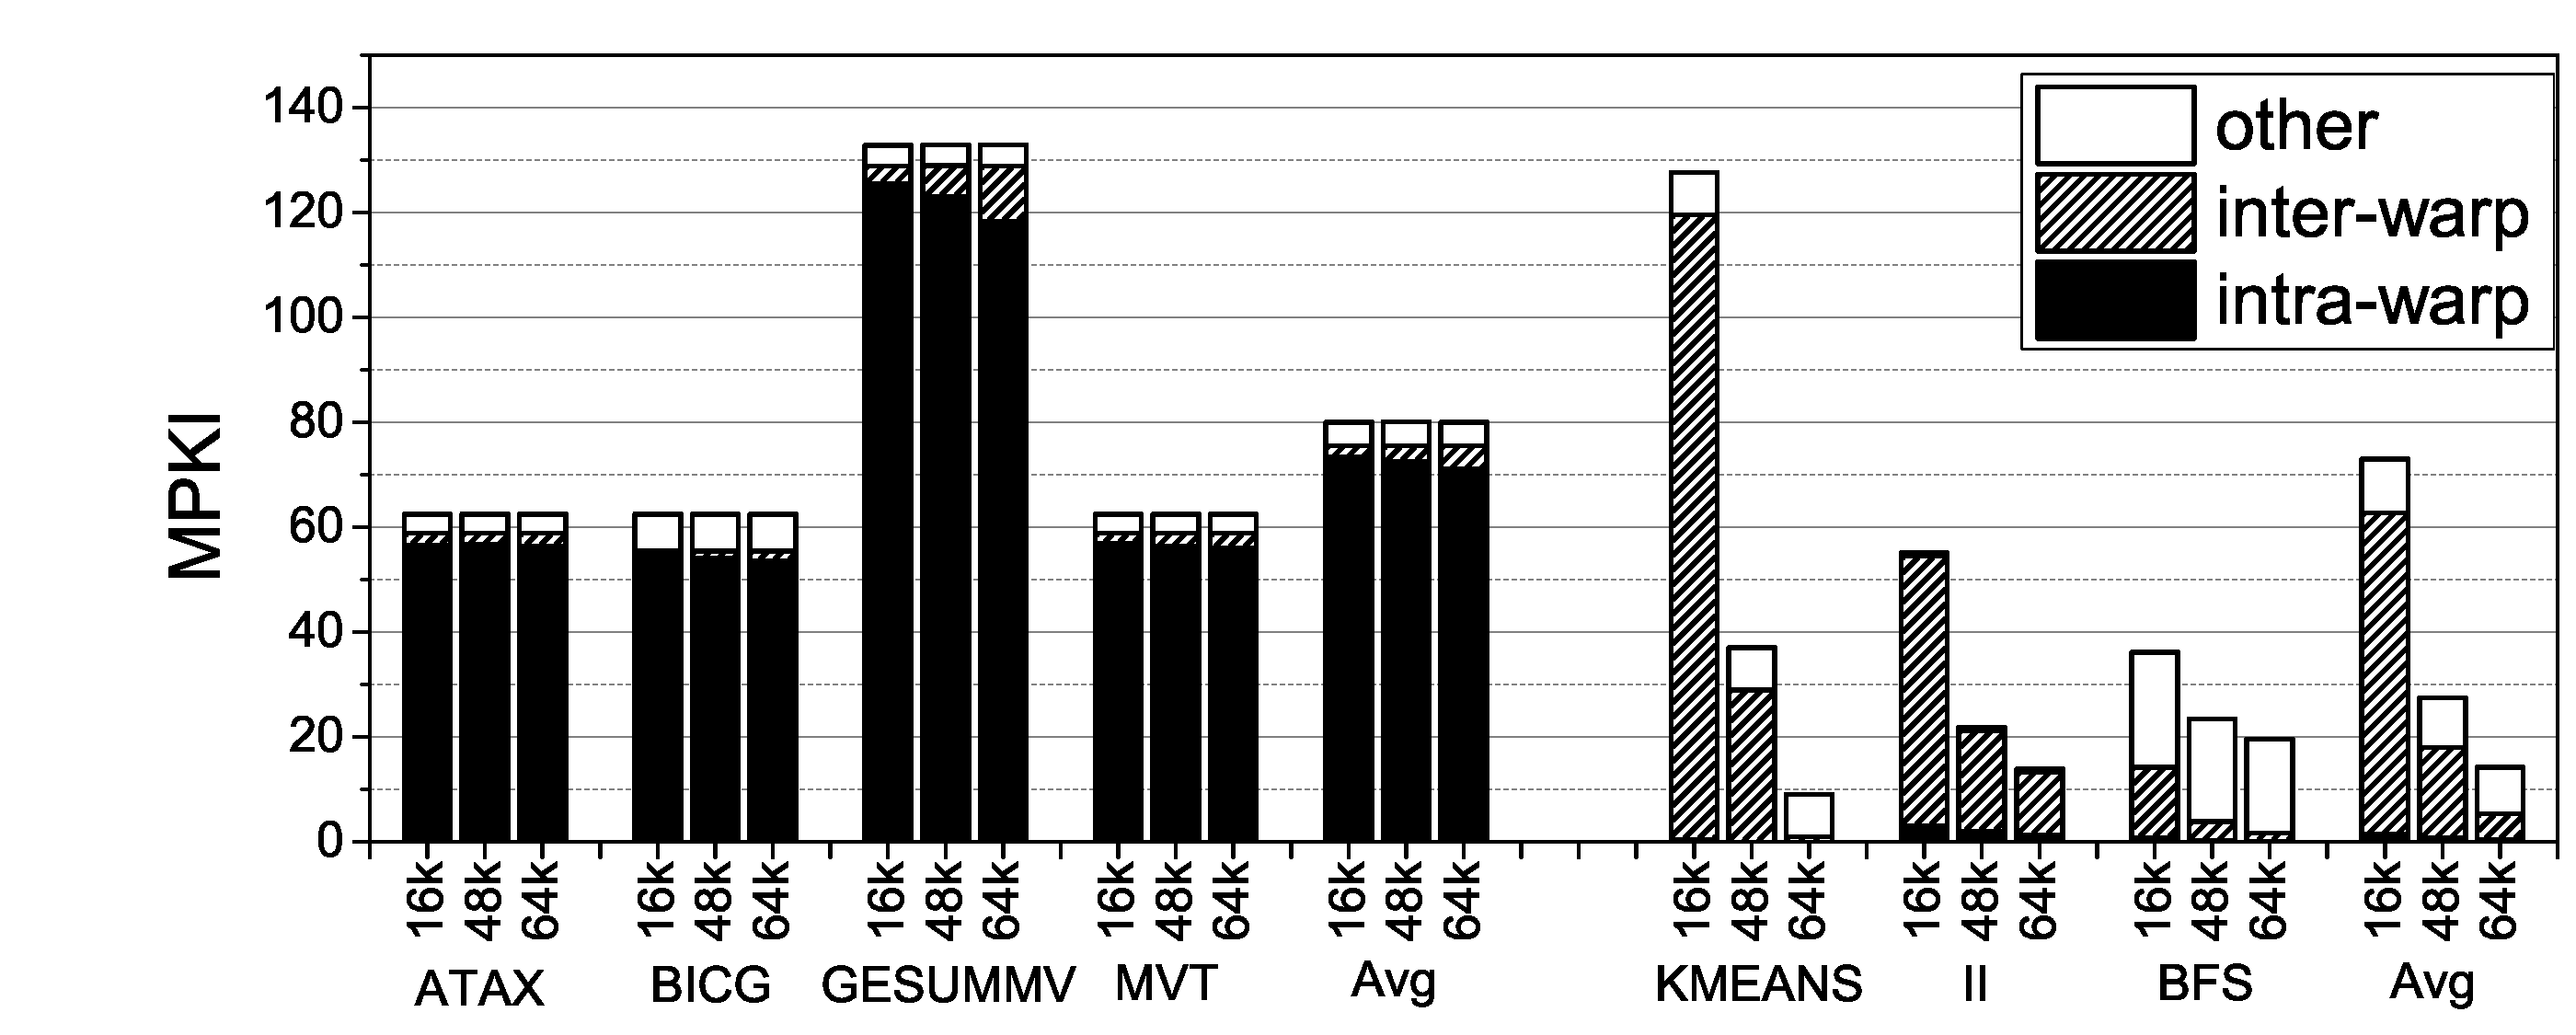
\epsfig{file=figs/mpki.eps,angle=-0,width=0.45\textwidth,clip=}
\end{center}
\vspace{-10pt}
\caption{\textbf{Misses per thousand instructions (MPKI) of L1D cache with different cache size. Cache misses are categorized into intra-warp contention, inter-warp contention and other (pure misses). For heavy memory intensive benchmarks, the misses mainly comes from intra-warp contention and changes very little with enlarged cache size. For moderate memory intensive benchmarks, the misses mainly comes from inter-warp contention and drops significantly with larger cache size.\label{fig:mpki}}}
%\vspace{-5pt}
\end{figure}

\begin{figure}
\begin{center}
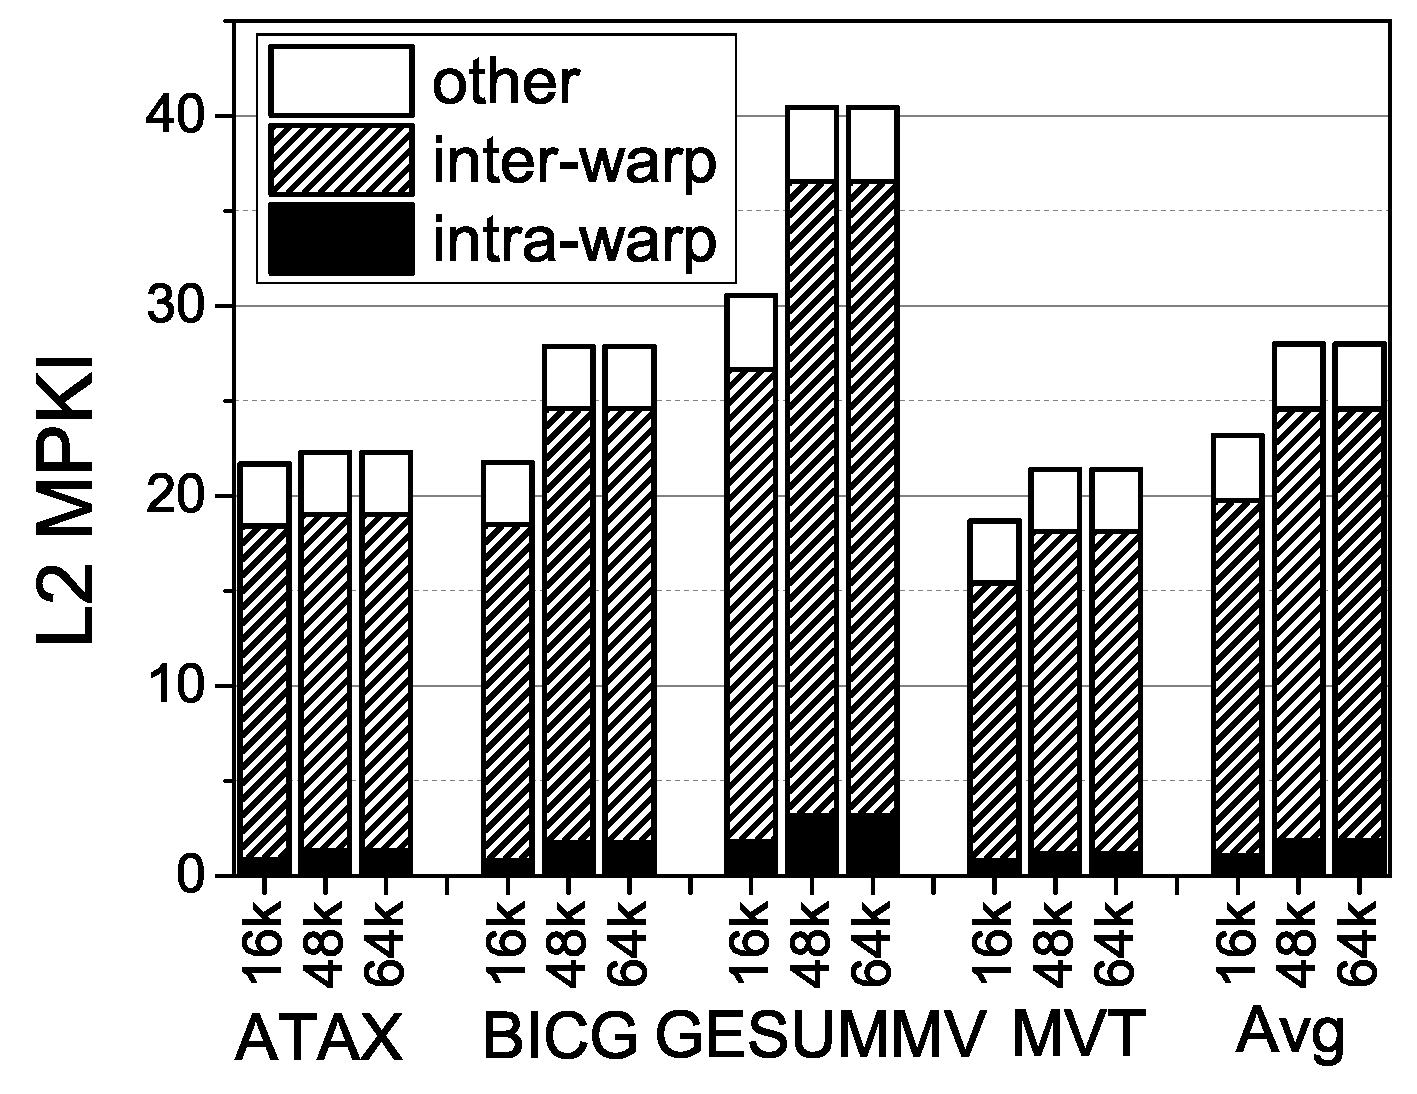
\epsfig{file=figs/l2_mpki.eps,angle=-0,width=0.25\textwidth,clip=}
\end{center}
\vspace{-10pt}
\caption{\textbf{ Misses per thousand instructions (MPKI) of L2 cache across memory intensive benchmarks with different L1D cache size. With a significantly larger size compared to L1D cache, the misses in L2 cache mainly comes from inter-warp contention. \label{fig:l2_mpki}}}
%\vspace{-5pt}
\end{figure}


\begin{figure}
  \begin{center}
    \mbox{
      \subfigure[\label{fig:swl_l1}]{\scalebox{0.22}{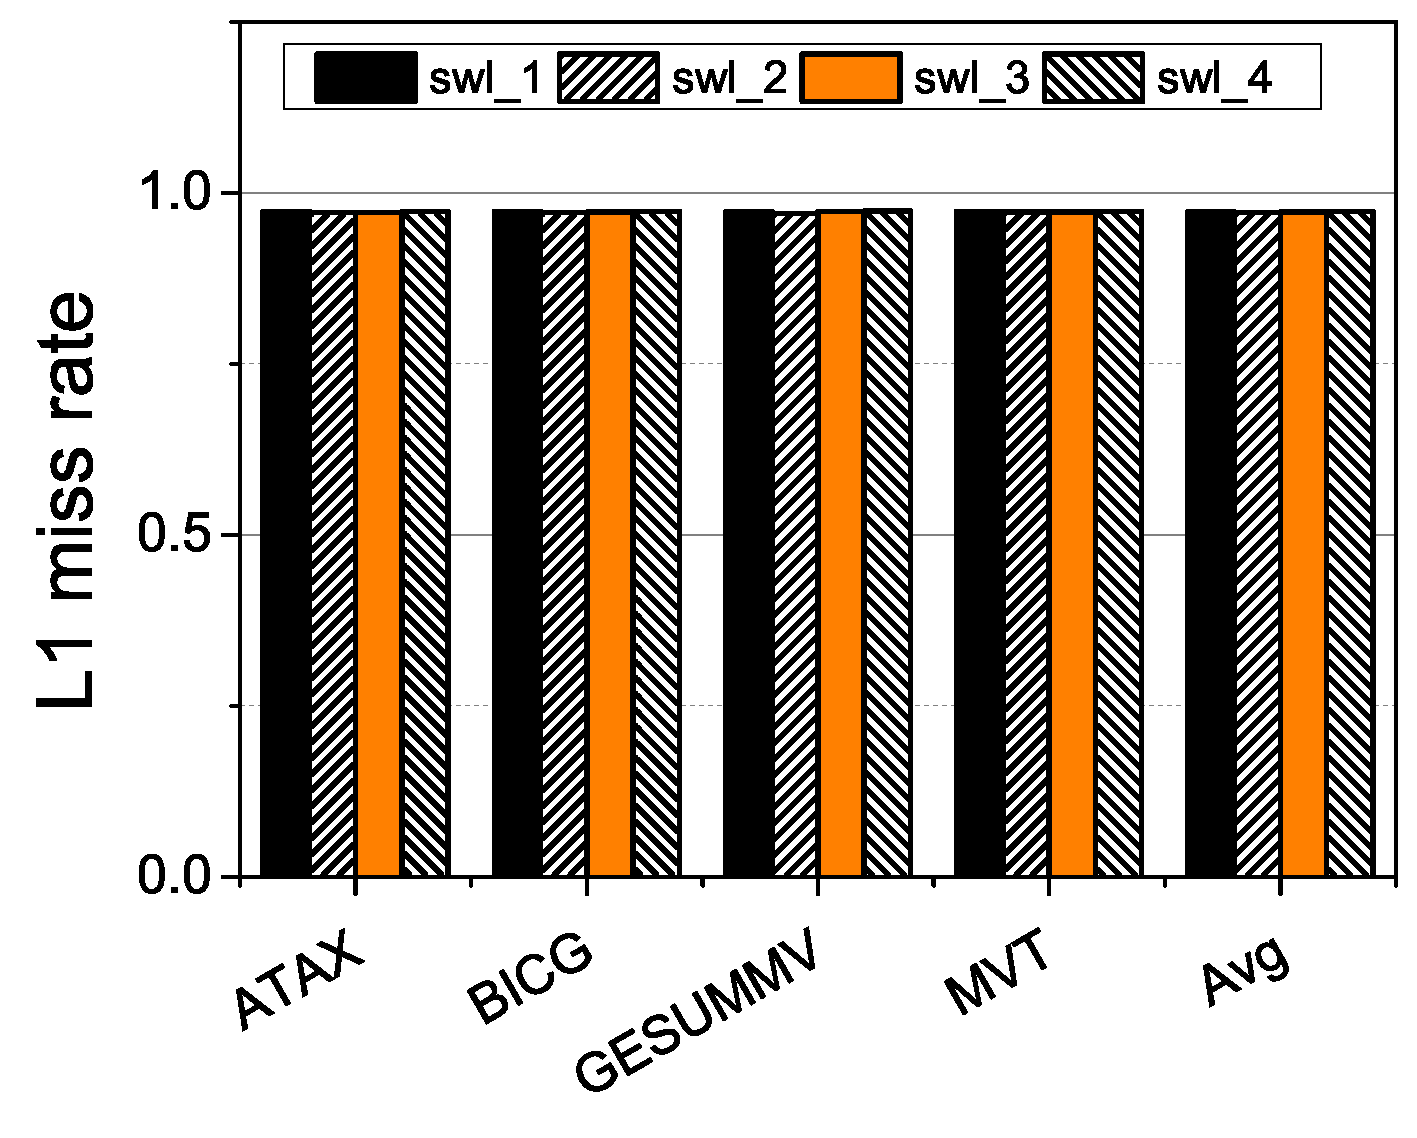
\epsfig{file=figs/swl_l1.eps,angle=-0,width=1\textwidth,totalheight=5.5in,clip=}}} \quad
      \subfigure[\label{fig:swl_l2}]{\scalebox{0.22}{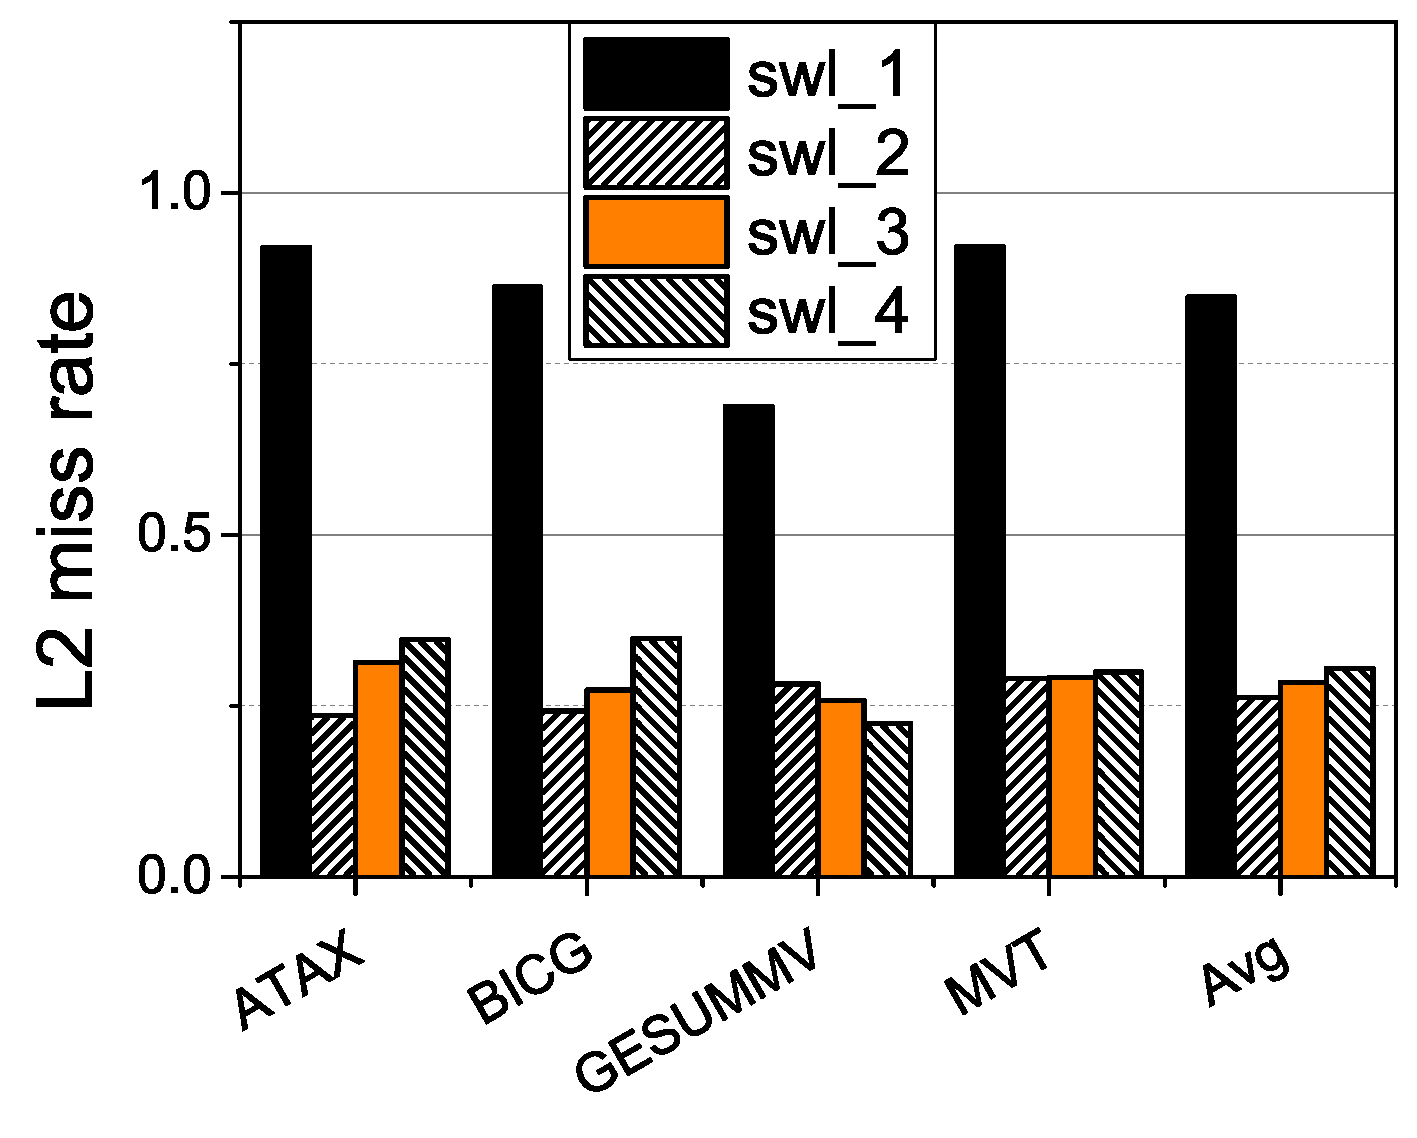
\epsfig{file=figs/swl_l2.eps,angle=-0,width=1\textwidth,totalheight=5.5in,clip=}}}\quad
    }
\end{center}
\vspace{-10pt}
\caption{\textbf{(a) L1D miss rate with SWL scheduler. With different number of active warps, the L1D miss rates are similar, because the cache size too small to accommodate the data for even a single warp. (b) L1D miss rate with SWL scheduler. The lowest miss rate is achieved when the number of active warps is less than the maximum except for GESUMMV, whose input size is smaller than other three benchmarks.}}
\vspace{-15pt}
\end{figure}

To show the significance of the L1D cache contention issue, we performed a simulation-based study using a cycle-level GPGPU simulator \cite{bakhoda2009analyzing}. In this work, we implement three different L1D cache sizes, i.e., the configurable cache size in Fermi architecture (16KB and 48KB) and a larger size of 64KB to show the potential performance. As shown in Figure \ref{fig:mpki}, intra-warp contention can be responsible for majority of the misses in the L1D cache for several data intensive workloads (i.e., ATAX, BICG, GESUMMV and MVT\cite{grauer2012auto}, with scaled down input size \cite{jia2014mrpb}). Even with a larger 48KB or 64 KB L1D cache, intra-warp contention is still the main cause of the cache misses. One can observe from this figure that, with 16KB L1D cache, while misses per thousand instruction (MPKI) caused by inter-warp contention accounts for only 2.7\% of total misses, 91.7\% of total MPKI, on average, is caused by intra-warp contention. Even with a larger 64KB L1D cache, intra-warp contention is responsible for 88.8\% of the total cache misses, while inter-warp contention only contributes 5.6\%. Due to the insensitivity of contention to the L1D cache size, we classify this kind of benchmarks as \textit{heavy memory intensive} benchmarks.

It should be noted that, for other workloads (i.e., BFS, KMEANS \cite{che2009rodinia} and II \cite{he2008mars}), even though majority of the cache misses are contributed by the inter-warp contentions with a small 16KB L1D cache, this challenge can be simply addressed if the L1D cache can be made larger. As one can see from Figure \ref{fig:mpki}, once the cache size is enlarged to 48KB and 64 KB, the inter-warp contention is largely reduced by 71.8\% and 92.1\%, respectively. As the cache contention can be reduced significantly by utilizing larger size L1D cache, we categorize this kind of benchmarks as \textit{moderate memory intensive} benchmarks.

%enough to accommodate all the data requested by the single warp. This is because, such data-intensive workloads also have the characteristic of large data reuse. Figure \ref{fig:l1_hit} shows the number of cache hits if we enlarge the L1D cache size. As we can see from this figure, 94.7\% cache hits of the data-intensive workloads can come from intra-warp, which indicated that the data are referenced multiple times by the same warp.

%In this work, we classify this kind of workloads to have \textit{L1-level intra-warp locality}, which means their performance can be significantly improved once the repeated data request can always be served from the L1D cache.

\noindent\textbf{Cache contention in L2}: In contrast to the L1D GPU cache, the shared L2 cache is significantly larger (e.g., 768KB in Fermi architecture \cite{nvidia2009nvidia}), and therefore it has the potential to accommodate data requested by multiple warps. As in the data-intensive \textit{ATAX} example, data requested by one entire warp is 256KB (2048*32*4), which is much larger than the L1D cache size and thus cannot be fully contained in L1D cache. However, it is less than the L2 cache size, and thus can be accommodated in L2 cache if there is not inter-warp contention at L2-level. As illustrated in Figure \ref{fig:l2_mpki}, the misses in L2 cache mainly comes from inter-warp contention. Since the L2-level inter-warp contention can come either from warps within the same SM or the warps across different SMs, we classify this kind of contention in L2 cache as \textit{L2-level interference}. One can learn from this observation that even though the intra-warp contentions cannot be avoided in L1D cache, \textit{the repeated data requests from the same warp can always hit on the shared L2 cache in the ideal case where the L2 cache can accommodate the data for a whole warp and there is no L2-level interference}. That is, although the L2 cache only have a few times more bytes per thread than the L1D cache dose when all SMs are fully utilized, once the number of active warps decreases, L2 cache has the potential to accommodate the entire data requested by fewer warps, and thus allocate more space for each thread.

As illustrated in Figure \ref{fig:gpu}, the shared L2 cache sits behind the interconnection network, which results in a notably longer latency (hundreds of cycles \cite{wong2010demystifying}) than the private L1D cache accesses. Because of this, only sporadic attention has been paid to improve its performance. However, our study shows that, instead of directly improving the L1D cache performance, sacrificing the L2 cache latency to avoid even longer DRAM accesses can significantly improve the overall GPGPU performance in cases where cache misses cannot be avoided in L1D cache due to intra-warp contention issue.

\subsection{Warp Scheduling}

In order to hide the latency of the underlying memory accesses, a hardware-based warp scheduler selects/issues a ready warp from a warp list following a specific scheduling policy, and try to improve the computation throughput. We now look into the three categories of warp scheduling policies that are commonly used in modern GPU architectures.

\remark{not implemented, should I?}
\noindent\textbf{Loose Round-Robin Scheduling (LRR)}: In this policy, multiple warps are ordered in the warp list based on their warp ID, and their executions are prioritized to be scheduled in a round-robin order. If the warp at the head of the list cannot be issued in the current cycle due to a long memory latency, it is logically moved to the end of the warp list, and the next warp in the list will get the highest priority.
While LRR has the advantage of simple implementation, it does not consider the cache performance for most part, and thus can cause higher performance degradation compared to the other, more advanced schedulers; particularly when executing memory intensive applications.

\noindent\textbf{Greedy-then-Oldest Scheduling (GTO)}: GTO priorities the oldest warp and runs it until it is stalled due to some long latency operation such as DRAM memory fetch. The age of a warp depends on the time it is assigned to the core. In this scheduling policy, if multiple warps have been assigned to a target core at the same time, a higher priority will be given to the one with the smaller thread IDs \cite{rogers2012cache}. As GTO always gives the higher priority to older warps, it guarantees that such older warps have more chances to exclusively access the underlying memory, which in turn can exhibit better performance than LRR.
 %However, if the warps contending for L1D cache are among the oldest ones assigned to the core, GTO still fails to handle this situation.

\noindent\textbf{Cache-Locality-Aware Scheduling (CLA)}: Several cache-locality-aware warp scheduling policies have being proposed in recent years in order to alleviate the long memory latency, such as the Two-Level Warp Scheduling \cite{narasiman2011improving}, Prefetch-aware Warp Scheduling \cite{jog2013orchestrated}, OWL scheduler \cite{jog2013owl} and Cache-conscious Wavefront Scheduling (CCWS) \cite{rogers2012cache}. This type of dynamic warp scheduling strategies are designed for reducing the L1D cache misses for cache sensitive applications by determining how many and which warps should be executed based on the memory access behavior at runtime. Specifically, in this work, we implement CCWS as a comparison, which is devised based on the observation that the majority of the data reuse behavior behind the highly cache-sensitive benchmarks comes from the same warp, that is, those benchmarks exhibit L1-level intra-warp locality. Once such L1 level intra-warp locality is detected for certain warps, these warps will be given more exclusive access to the L1D cache by stalling the warps with less L1 level intra-warp locality. The goal here is to reduce the inter-warp contention, and increase the L1 cache hit by throttling the number of active warps to some extend.

It should be noted that, for benchmarks that exhibit memory requests of particularly large sizes, repeated data reuse from even a single warp can generate large L1D cache misses. Unfortunately, none of these three scheduling policies can effectively improve the L1D cache performance in such a scenario.


\section{Interference-Aware Scheduling}

\subsection{Overview of iWarp}

The cache-locality aware scheduling methods prioritize the warps experiencing high L1-level intra-warp locality in an attempt to reduce the ``inter-warp contention" caused by many cache accesses of multiple active warps within a streaming multiprocessor. However, as shown in Figure \ref{fig:mpki} we observe that, for heavy memory intensive benchmarks, the majority of the misses in the L1D cache are generated by the repeated data requests from the same warps (i.e.,``intra-warp contention"). In other words, even with a single active warp, this intra-warp cache contention cannot be reduced effectively by the existing warp schedulers -- we demonstrate this in Figure \ref{fig:swl_l1}, where we apply static wavefront scheduling (SWL) \cite{rogers2012cache} scheme, where the limit on the number of warps/wavefronts are specified by the programmer, to the heavy memory intensive benchmarks with 16KB L1D cache. As one can observe from Figure \ref{fig:swl_l1}, even with the limit of only one active warp for each scheduler, the L1D cache miss rate is similar to when all warps are active (in this case, four warps for each scheduler). One of the insights behind this work is that, \textit{such intra-warp contention problem can actually be addressed at the L2 level, if one can take advantage of the larger size of L2 cache to get a higher cache hit rate at L2-level}. That is, reducing the inter-warp contention shown in Figure \ref{fig:l2_mpki} as much as possible to obtain a higher L2 hit rate, and thus avoid the long DRAM memory access. Motivated by this, we propose a cache interference-aware dynamic scheduling technique, iWarp, which can alleviate the L2-level interference and improve L2-level intra-warp locality. Even though L2 cache accesses exhibit relatively long latency, the data requested from the same warp can be served from the L2 cache, rather than having to retrieve it from the underlying global memory (DRAM), which in turn can save more than hundreds of cycles. In addition to hiding the long latency of accessing the DRAM, which can in turn improve the overall performance, our proposed iWarp can also increase the GPU's energy efficiency.

Further, the most conventional warp schedulers do not consider the cache interference between warps while choosing which warp is to be stalled. As a result, two warps that both exhibits L1-level intra-warp locality can contend for acquiring the same cache blocks, which can unfortunately generate many cache misses. In contrast, our proposed iWarp detects the cache contention between warp pairs, and stalls one of them to leave the other with more cache blocks in L2. In this way, iWarp can ensure that the data requested by the currently executing warp can reside in the L2 cache with fewer interference from other warps, and thus guarantee a high hit rate in the L2 cache.

Figures \ref{fig:ipc_potential} and \ref{fig:l2_potential} illustrate a motivational example for our proposed scheme and the rationale behind it, respectively.
Specifically, Figure \ref{fig:ipc_potential} shows GPU performance for particularly data-intensive workloads using LRR, and varying L2 cache sizes. One can observe that, with an unlimited L2 cache size, those workloads have 86.7\% performance improvement over the L2 cache configuration with a default GPU cache size (786 KB). Figure \ref{fig:l2_potential} demonstrates that, the reason behind this performance improvement is a sharp decline in L2 cache misses, which can be up to 97.0\% compared to the baseline L2 cache size. Since, physically increasing the size of L2 cache can be expensive and hard to implement, our iWarp reduces the L2 cache misses by throttling the number of active warps that exhibit interference of many cache accesses which lead to significant cache thrashing. In this way, our iWarp can leverage the baseline L2 configuration without any architectural modification, and can approach the aspired behavior of an unlimited L2 cache.


\subsection{Scheduling Strategy}

\subsubsection{L1-level}

\begin{figure}
\begin{center}
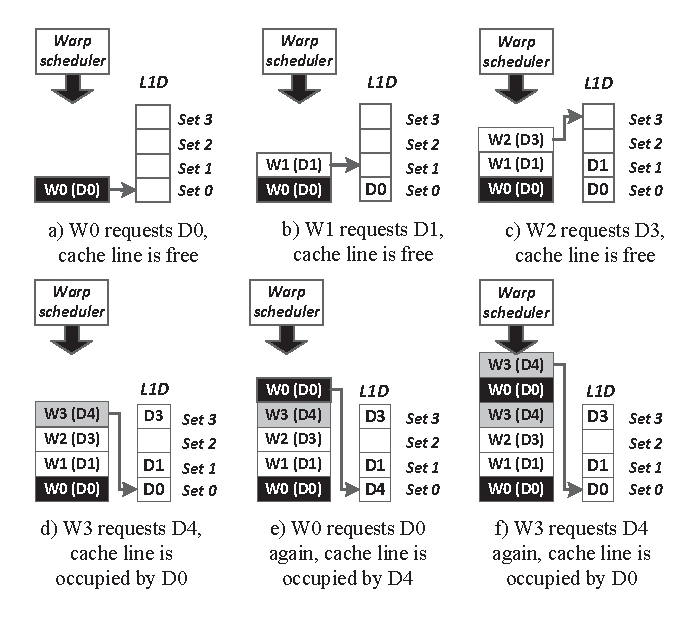
\epsfig{file=figs/l1_contention.eps,angle=-0,width=0.45\textwidth,clip=}
\end{center}
\vspace{-10pt}
\caption{\textbf{Illustration of inter-warp contention in L1D cache. Data D0 and D4 that are rereferenced by warp W0 and W3, respectively, have inter-warp contention with each other.\label{fig:l1_contention}}}
%\vspace{-5pt}
\end{figure}

\begin{figure}
\begin{center}
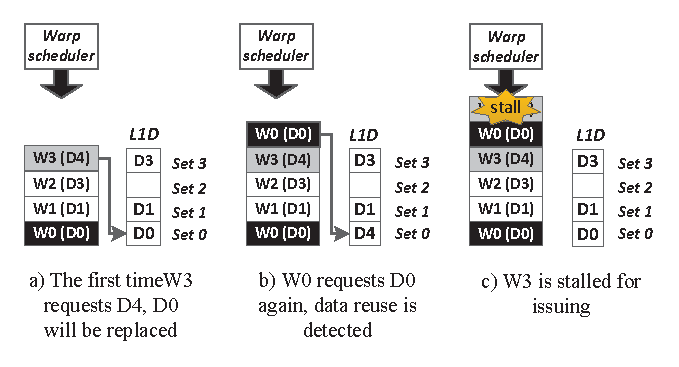
\epsfig{file=figs/iWarp_l1.eps,angle=-0,width=0.45\textwidth,clip=}
\end{center}
\vspace{-10pt}
\caption{\textbf{Illustration of iWarp working scheme on L1-level using the example in Figure \ref{fig:l1_contention}. The first time warp W3 requests data D4, D0 in cache set0 will be replaced. Then when W0 requests D0 again, data reuse of D4 is detected, so as the contention between W0 and W3. iWarp stalls loading W3, and thus further data reuse of D0 from W0 will hit on L1D cache.\label{fig:iWarp_l1}}}
%\vspace{-5pt}
\end{figure}

To make a better scheduling decision about eliminating the cache interference, our iWarp is capable of capturing the underlying cache contention by recording which warps send the memory requests. Once a pair of warps in the same SM is detected to have inter-warp contention between each other, our iWarp assigns the current executing warp priority to access L1 cache by stalling the other warp. In other words, for the current executing warp, our iWarp stalls the warp that causes the latest cache contention with it.

Figure \ref{fig:l1_contention} shows an example that illustrate the inter-warp contention caused by data reuse within a single SM in L1-level. For simplicity, we assume that there are four active warps, four sets in L1D cache and each set has one cache line. All cache lines are free at the initial state. W0(D0) means warp0 requests for data D0, and the arrow shows the data mapping to the cache line. As is shown by Figure \ref{fig:l1_contention} a), b) and c), the first three data requests do not cause any contention since the corresponding cache lines are free. When W3 requests for D4 in Figure \ref{fig:l1_contention} d), the corresponding cache line is occupied by D0 which was requested by W0. Therefore D0 will be replaced by the latest requested D4. When W0 is issued later on and requests for D0 again in Figure \ref{fig:l1_contention} e), conflict miss occurs since the cache line is occupied by D4. Similar situation happens when W3 is issued and requests for D4 again as is shown in Figure \ref{fig:l1_contention} f).

iWarp aims to detect the wrap pair that are contending for the same cache line (W0 and W3 in previous example in Figure \ref{fig:l1_contention}), and stall one of them to leave the other more cache space so that the following data reuse of the remaining active warp can always hit on cache.

The modified cache structure that is able to detect the cache interference cause by data reuse is given in Section \ref{sec:arch},

The following example illustrates the core strategy of our iWarp. Figure \ref{fig:iWarp_l1} a) corresponds to Figure \ref{fig:l1_contention} d) when W3 requests for D4 for the first time, and D0 will be replaced. In Figure \ref{fig:iWarp_l1} b), W0 requests for D0 again but causes cache miss since D0 has been replaced by D4. In such case, iWarp detects the data reuse of W0 and stops W3 for further issuing as is shown in In Figure \ref{fig:iWarp_l1} c). Therefore, further data reuse of D0 by W0 can hit on cache. In addition, when W0 finishes executing or the cache contention. That is, when W0 does not request for data in cache set0 any more, W3 is reactivated, and its reuse of data D4 can hit on cache without the conflict from W0. In such way, iWarp reduces the L1 miss rate when the misses mainly come from inter-warp contention.

\subsubsection{L2-level}


\begin{figure*}
  \begin{center}
    \mbox{
      \subfigure[Without L2-level interference. \label{fig:l2_1}]{\scalebox{0.32}{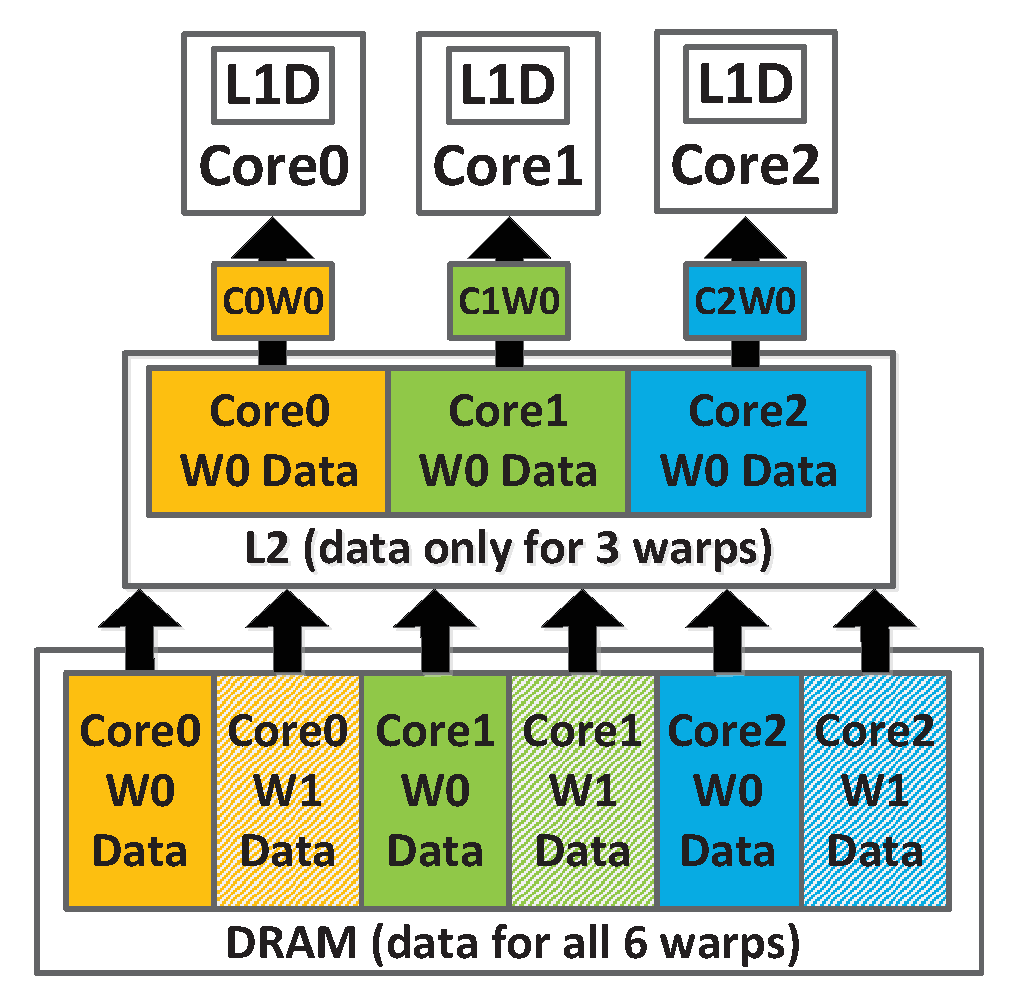
\epsfig{file=figs/l2_1.eps,angle=-0,width=1\textwidth,totalheight=7.2in,clip=}}} \quad
      \subfigure[With L2-level interference. \label{fig:l2_2}]{\scalebox{0.32}{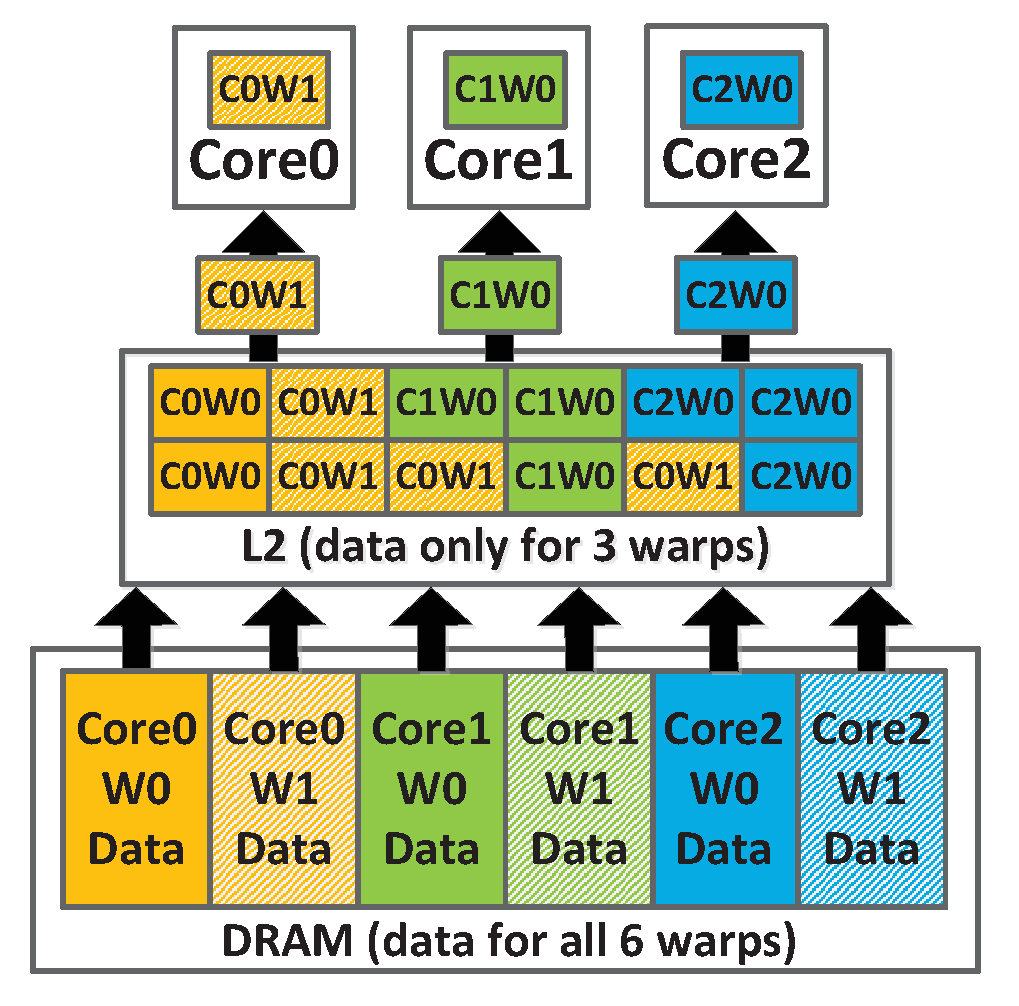
\epsfig{file=figs/l2_2.eps,angle=-0,width=1\textwidth,totalheight=7.2in,clip=}}}\quad
      \subfigure[L2-level interference eliminated. \label{fig:l2_3}]{\scalebox{0.32}{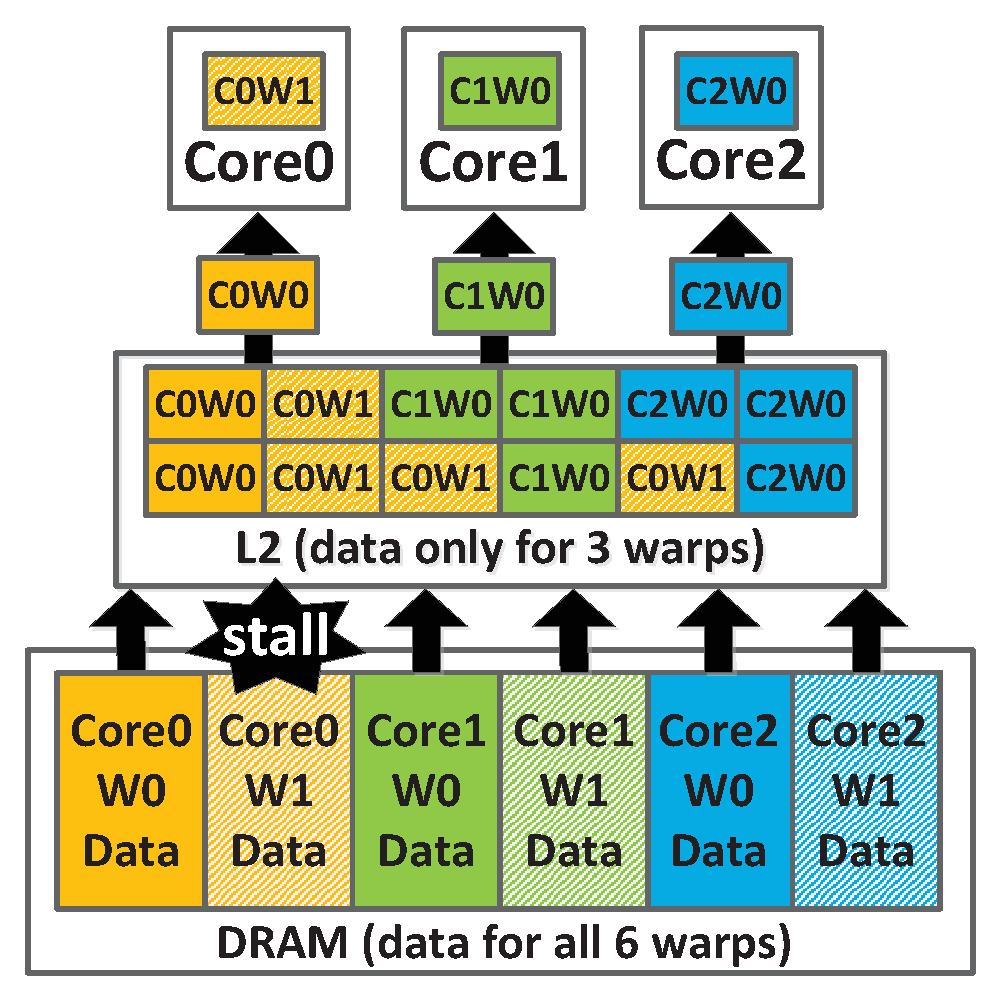
\epsfig{file=figs/l2_3.eps,angle=-0,width=1\textwidth,totalheight=7.2in,clip=}}}
    }
\end{center}
\vspace{-10pt}
\begin{center}
\caption{\textbf{A representative example of the cache contention problem and our iWarp scheduling strategies. (a) An ideal case where despite severe intra-warp contentions in L1D cache, there is no inter-warp contention in the L2 cache. Every data missed in the L1D cache can always hit in the L2 cache. (b) Newly requested data for warp1 in core0 (C0W1) occupies the cache blocks in L2, which introduces inter-warp contention in L2 cache. This contention causes L2 misses for other cores as their data has been replaced and can eventually be detected in core0. (c) Once the cache interference is detected, iWarp stalls the warp1 in core0, and the corresponding data will be stalled loading to L2 cache, which will reduce the L2 misses. \label{fig:l2}}}
\end{center}
\vspace*{-15pt}
\end{figure*}

In order to detect the L2-level interference, our iWarp needs to keep the history information for L2 cache. However, we propose to avoid such costly overhead by taking advantage of the large data reuse observed in GPU workloads, and detect the cache contention between warps from the smaller L1D cache instead. As a consequence, we can significantly reduce the hardware overhead for implementing iWarp. The key idea here is that, the data that sits in L1D cache also occupies L2 cache blocks. In other words, the data that is fetched to L2 cache will eventually be fetched to L1D cache. As such, the L2-level interference can actually be detected in L1D cache as inter-warp contention, and thus no more further modification is needed. The following example illustrates the key idea of our iWarp at L2-level.

Figure \ref{fig:l2} demonstrates a simplified example of the cache contention problem observed for data-intensive GPGPU workloads. In this example, we assume that there are three cores, and each core has two active warps for the sake of brevity. The L1D cache in each core can only hold data for one-fourth of threads in a warp (i.e., eight threads), while the L2 cache is able to maintain all the data for three warps. As a result, data of all six warps will contend for the limited L2 cache blocks. For L1D cache, as shown in Figure \ref{fig:l2_1}, when the requested data for one warp is fetched from L2 to L1D cache, the incoming data will cause frequent data replacements in L1D cache due to the data being larger than the cache capacity. For example, since data for warp0 in core0 (C0W0) is four times larger than the L1D cache size, newly incoming data will replace the data for the same warp that already occupies L1D cache blocks. Due to the large data reuse characteristic in the data-intensive workloads, such frequent data replacements in turn can introduce a high L1D miss rate.

Figure \ref{fig:l2_1} represents an ideal case where, the entire data requested by the currently executing warp can be found in the L2 cache for each core. As a result, irrespective of the huge L1 misses caused by intra-warp contention, L2 fully catches the intra-warp locality and can generate cache (excluding the cold start) hits in most cases, which in turn can avoid the long latency of accessing the slow DRAM-based GPU memory.

Figure \ref{fig:l2_2} illustrates the situation regarding L2 cache interference. Once the executing warp in core0 switches to warp1 due to some long latency operation of warp0, a portion of the blocks in L2 cache will be replaced by the newly requested data. Since the data for core1 and core2 is replaced, the future requests from these two cores will introduce L2 cache misses, which will result in time-consuming data extraction from the underlying DRAM. Further, once the data is fetched from the DRAM for core1 and core2, the replacement operation in L2 cache can aggravate the cache interference.

The detection of cache interference in our iWarp scheduler is triggered when core0 switches back to executing warp0 from Figure \ref{fig:l2_2} to Figure \ref{fig:l2_3}. Because of the data reuse feature, warp0 will request for the same data as in its previous execution. In Figure \ref{fig:l2_3}, the block in core0 indicates the old data ``C0W1" in L1D cache before it is replaced by the new incoming data ``C0W0". Upon the data replacement, by figuring out that the current requested data ``C0W0" \textit{was} in L1D cache, iWarp can identify this cache miss as a result of inter-warp contention. That is, the L2-level interference eventually propagated to L1-level and shown as the form of inter-warp contention. Once warp1 in core0 that introduces the interference is stalled as shown in Figure \ref{fig:l2_3}, data ``C0W1" will stop loading from DRAM to L2 cache. In this way, the frequent data replacement problem in L2 can be alleviated, and more L2 cache blocks can be allocated to the other executing warps, which can in turn reduce L2 misses.

In real GPU workloads, as there are many more active warps and much larger data set, the cache interference can be significantly more severe, which requires intensive levels of warp scheduling for capturing L2-level intra-warp locality. In summary, even when the L1D cache misses cannot be avoided for data intensive workloads due to the small cache size, our iWarp aims to keep the requested data in L2 for a longer time by reducing the cache interference, so that the repeatedly requested data can hit on the L2 cache more frequently, improving overall performance.

\section{Scheduler Implementation}

\subsection{Cache Structure Modification}
\label{sec:arch}

\begin{figure}
\begin{center}
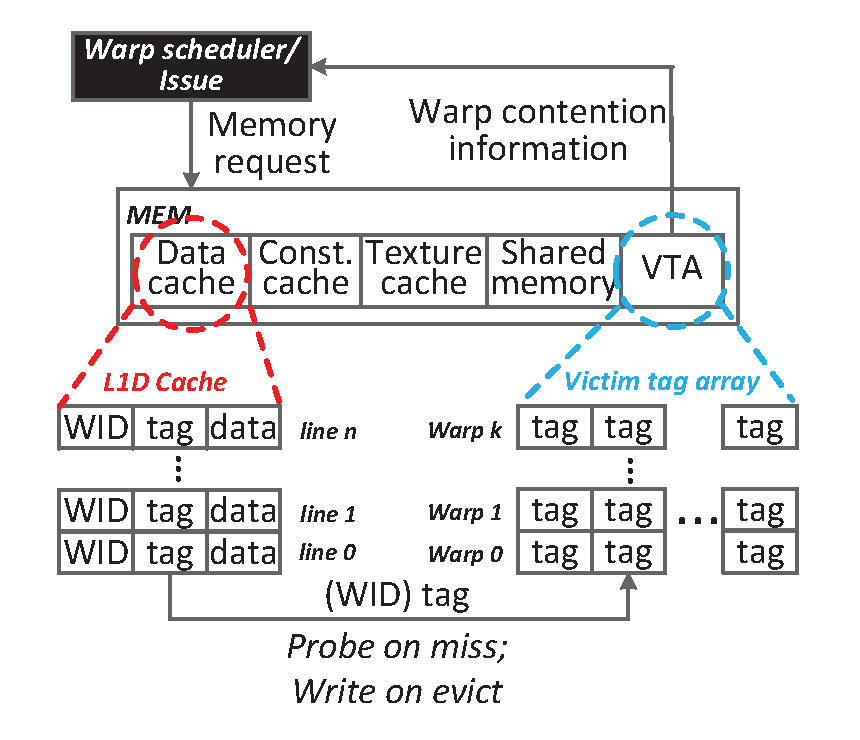
\epsfig{file=figs/vta.eps,angle=-0,width=0.35\textwidth,totalheight=2in,clip=}
\end{center}
\vspace{-10pt}
\caption{\textbf{Modified cache structure for our proposed iWarp scheme. A warp ID (WID) is added to each L1D cache line and a victim tag array (VTA) is introduced for each warp. The warp contention information is detected in VTA upon cache miss, and is fed back to the warp scheduler. \label{fig:vta}}}
\vspace{-15pt}
\end{figure}

To detect the both the L1 and L2-level interference through L1-level cache contention, we use the modified cache structure as shown in Figure \ref{fig:vta}. A \emph{warp ID (WID)} is added to each cache line of L1D cache in order to identify the warp reserving it. In addition, each warp is associated with a \emph{victim tag array (VTA)} in the memory unit. When a cache line is reserved on a cache miss, the warp ID associated with the cache line is written into the WID field. On the other hand, if a cache line is evicted from the L1D cache, the corresponding tag of that line is written into the victim tag array associated with that warp. In this way, VTA keeps the record of each warp's memory request history. Whenever there is a miss on the L1D cache, the VTA associated with the warp that sent the memory request is probed. If the requested tag is found in the VTA, it means that the currently executing warp generates a same data request as the one found in its request history. If the current miss is due to an inter-warp contention, the underlying L2 cache interference is detected. In this case, though there is little we can do to address the L1-level intra-warp locality due to the limited L1D cache size for heavy memory intensive workloads, our iWarp will leave more cache blocks for this executing warp in the L2 cache to mitigate the L2-level interference, and thereby catch the intra-warp locality in L2-level; which in turn can avoid the longer DRAM memory access.

\begin{figure}
\begin{center}
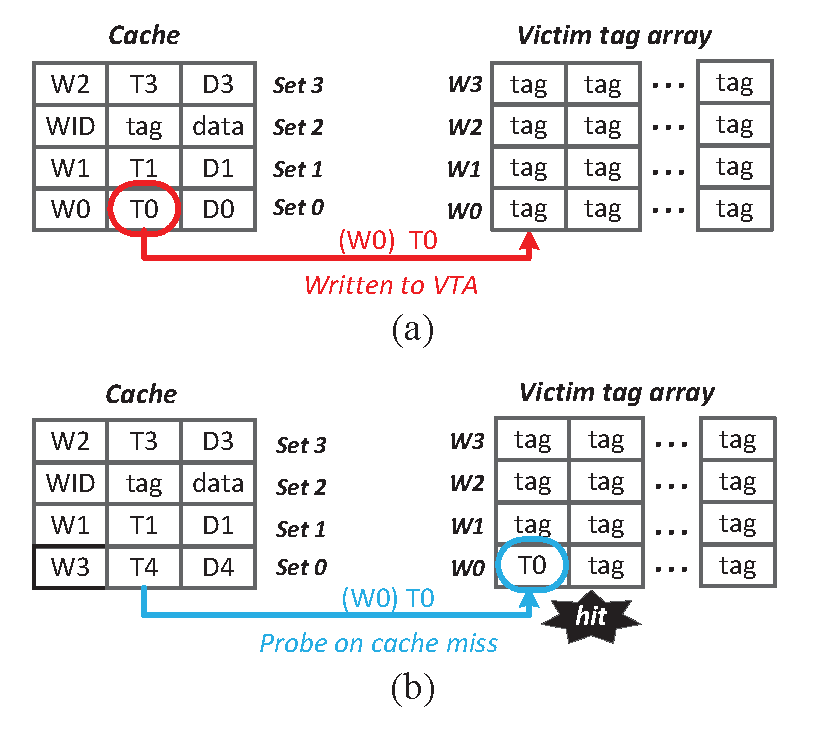
\epsfig{file=figs/vta_ex.eps,angle=-0,width=0.35\textwidth,totalheight=2in,clip=}
\end{center}
\vspace{-10pt}
\caption{\textbf{iWarp strategy details. (a) When a cache line is evicted from the L1D, its tag is written into the VTA portion that corresponds to the warp reserving it (marked using the WID). (b) Upon a cache miss, the requested data's tag is probed in the requesting warp's corresponding VTA. If the tag is found, a hit signal is generated. \label{fig:vta_ex}}}
\vspace{-15pt}
\end{figure}

An illustration of how the modified cache is employed in the case of Figure \ref{fig:iWarp_l1} is shown in Figure \ref{fig:vta_ex}. Figure \ref{fig:vta_ex}(a) illustrates when the data $D0$ for warp W0 is going to be replaced by W3's data $D4$ corresponding to Figure \ref{fig:iWarp_l1} a). Before the replacement, tag $T0$ is written to W0's portion of VTA. When W0 is issued and it requests for $D0$ again in Figure \ref{fig:iWarp_l1} b), W0's portion of VTA is probed, following the miss in L1 cache as shown in Figure \ref{fig:vta_ex}(b). Since $T0$ exists in VTA, a hit signal is generated, which indicates that the currently requested data $D0$ \textit{was} in the cache. And thus the inter-warp contention is detected.

%In addition, since this cache miss is identified as inter-warp contention in L1-level, it further indicates the cache interference has occurred in L2-level.

\subsection{Cache Interference Aware Scheduling}



\section{Evaluation}


\subsection{Methodology}
\label{sec:method}

\begin{table}
\begin{center}
\scriptsize
\begin{tabular}{|c|p{3.5cm}|}
\hline
No. of SMs & 15 \\ \hline
Warp size & 32 \\ \hline
No. of warp schedulers & 2 \\ \hline
No. of threads per SM & 1536 \\ \hline
L1D cache/Shared Memory per SM (i)& 16KB, 128B line, 4-way assoc./48KB \\ \hline
L1D cache/Shared Memory per SM (ii)& 48KB, 128B line, 6-way assoc./16KB \\ \hline
L1D cache/Shared Memory per SM (iii)& 64KB, 128B line, 8-way assoc./16KB \\ \hline
Unified L2 & 786KB, 128B line, 8-way assoc. \\ \hline
L1D policy & allocate on miss, local write-back, global write-through \\ \hline
L2 policy & allocate on miss, write back \\ \hline
\end{tabular}
\end{center}
%\vspace{-0.15 in}
\caption{\textbf{\label{tab:config}GPGPU-Sim configuration.}}
%\vspace{-0.25 in}
\end{table}

\begin{table}
\begin{center}
\scriptsize
\begin{tabular}{|c|c|c|}
\hline
Benchmarks & Description & Suite\\ \hline
\multicolumn{3}{|c|}{\textbf{Heavy memory intensive}}\\ \hline
ATAX & Matrix Transpose and Vector Multiplication & \cite{grauer2012auto}\\ \hline
BICG & BiCG Sub Kernel of BiCGStab Linear Solver & \cite{grauer2012auto}\\ \hline
GESUMMV & Scalar, Vector and Matrix Multiplication & \cite{grauer2012auto} \\ \hline
MVT & Matrix Vector Product and Transpose & \cite{grauer2012auto} \\ \hline
\multicolumn{3}{|c|}{\textbf{Moderate memory intensive}}\\ \hline
KMEANS & K-means Clustering & \cite{che2009rodinia} \\ \hline
II & Inverted Index & \cite{he2008mars} \\ \hline
BFS & Breadth First Search & \cite{che2009rodinia} \\ \hline
\end{tabular}
\end{center}
%\vspace{-0.15 in}
\caption{\textbf{\label{tab:benchmark}GPGPU benchmarks.}}
%\vspace{-0.25 in}
\end{table}

\subsection{Experimental Results}
\label{sec:result}


\subsubsection{Performance Analysis}
\label{sec:analy}

\begin{figure*}
  \begin{center}
    \mbox{
      \subfigure[16KB. \label{fig:16k_ipc}]{\scalebox{0.32}{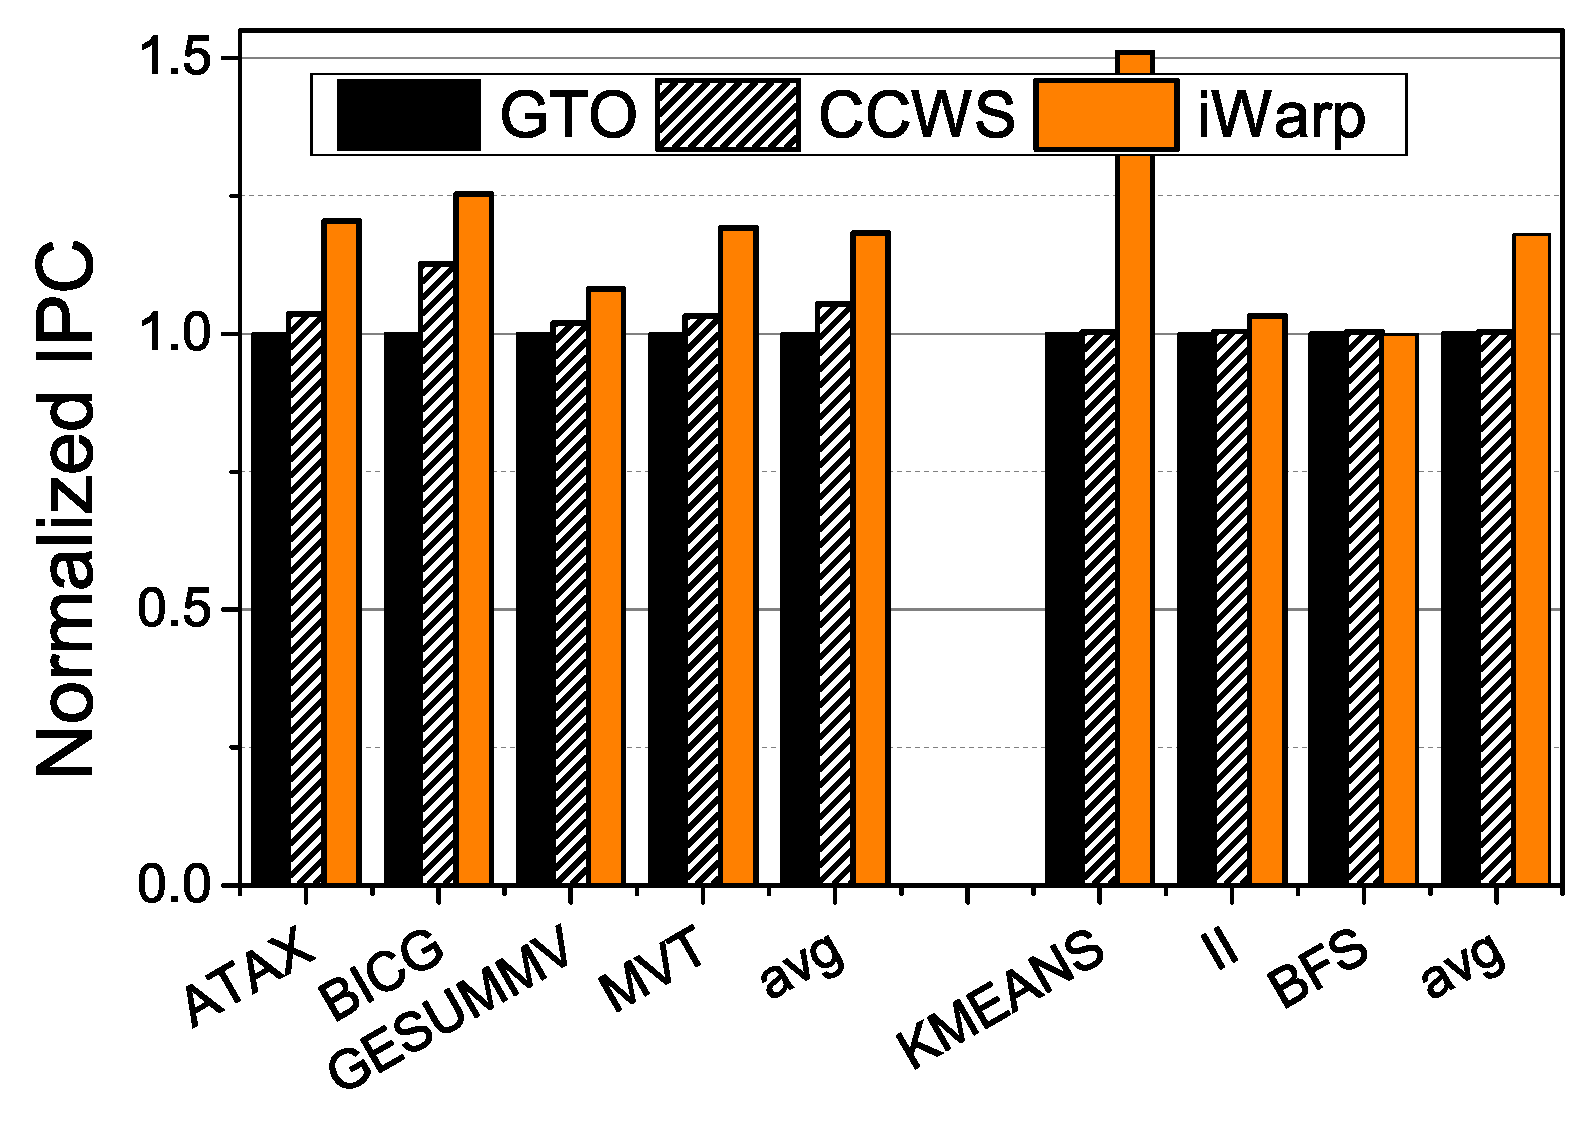
\epsfig{file=figs/16k_ipc.eps,angle=-0,width=1\textwidth,totalheight=5in,clip=}}} \quad
      \subfigure[48KB. \label{fig:48k_ipc}]{\scalebox{0.32}{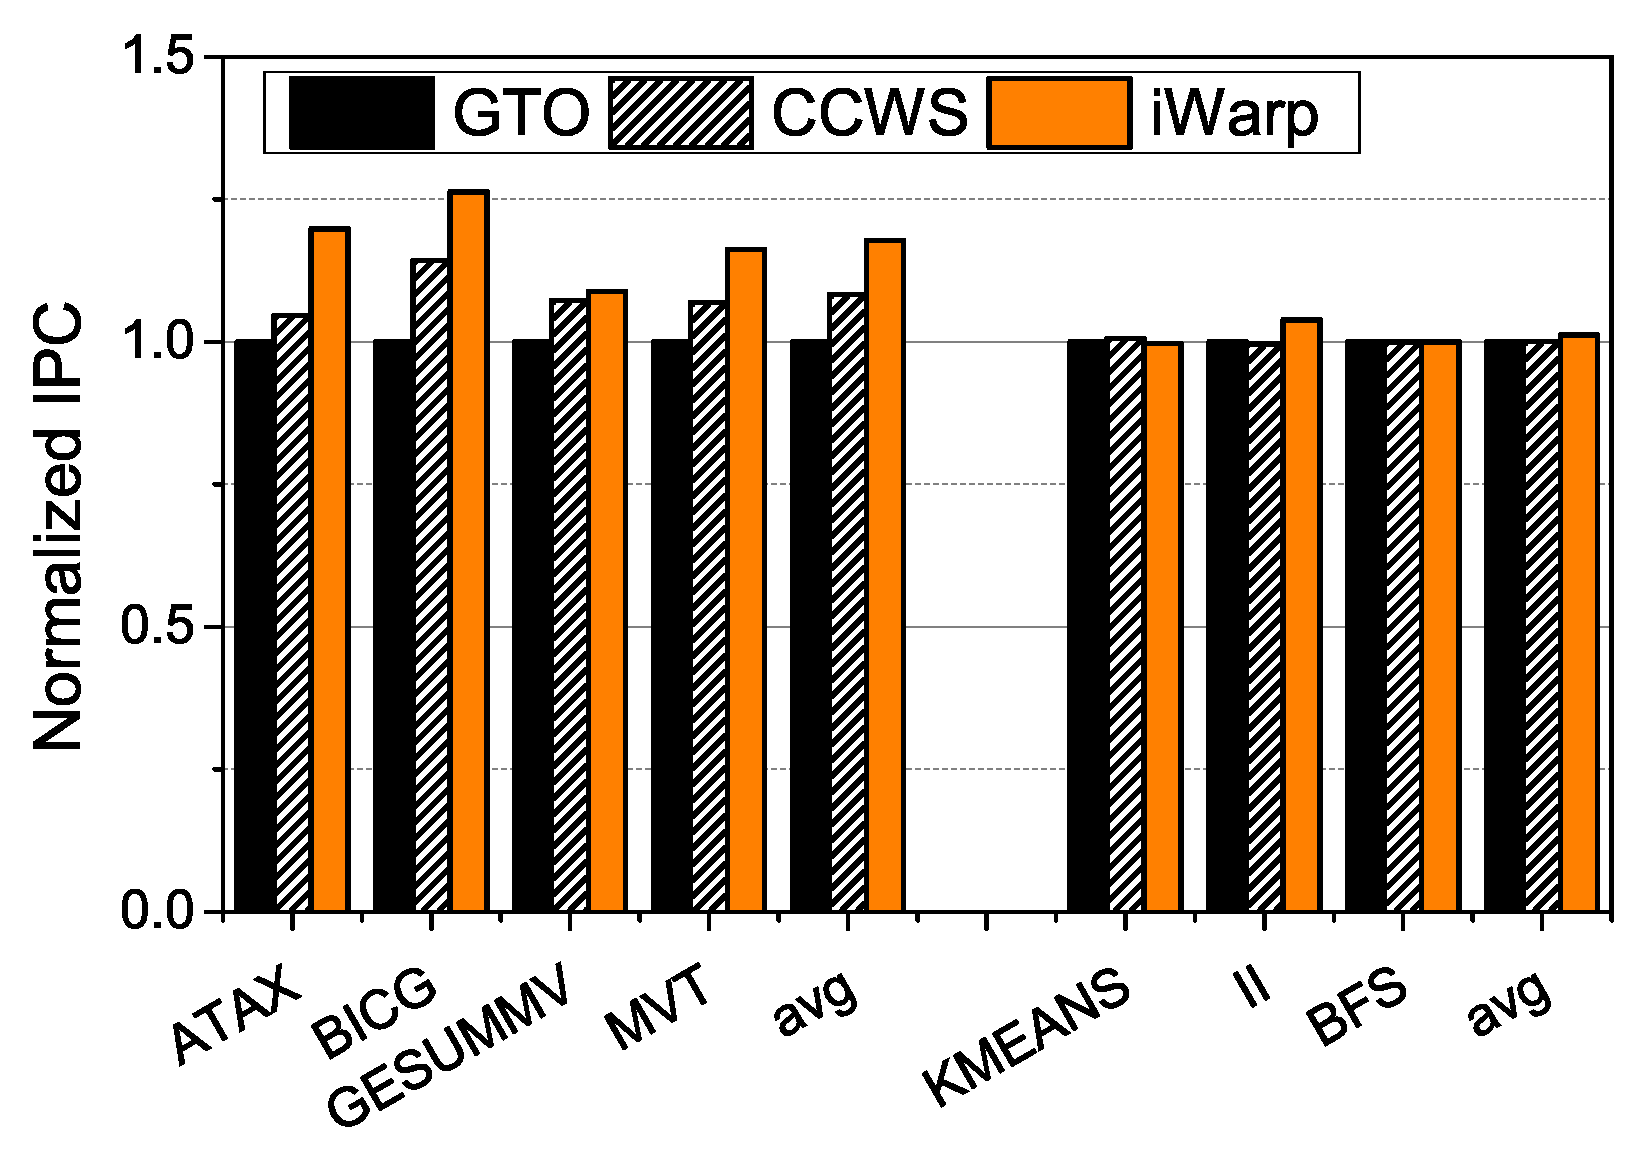
\epsfig{file=figs/48k_ipc.eps,angle=-0,width=1\textwidth,totalheight=5in,clip=}}}\quad
      \subfigure[64KB. \label{fig:64k_ipc}]{\scalebox{0.32}{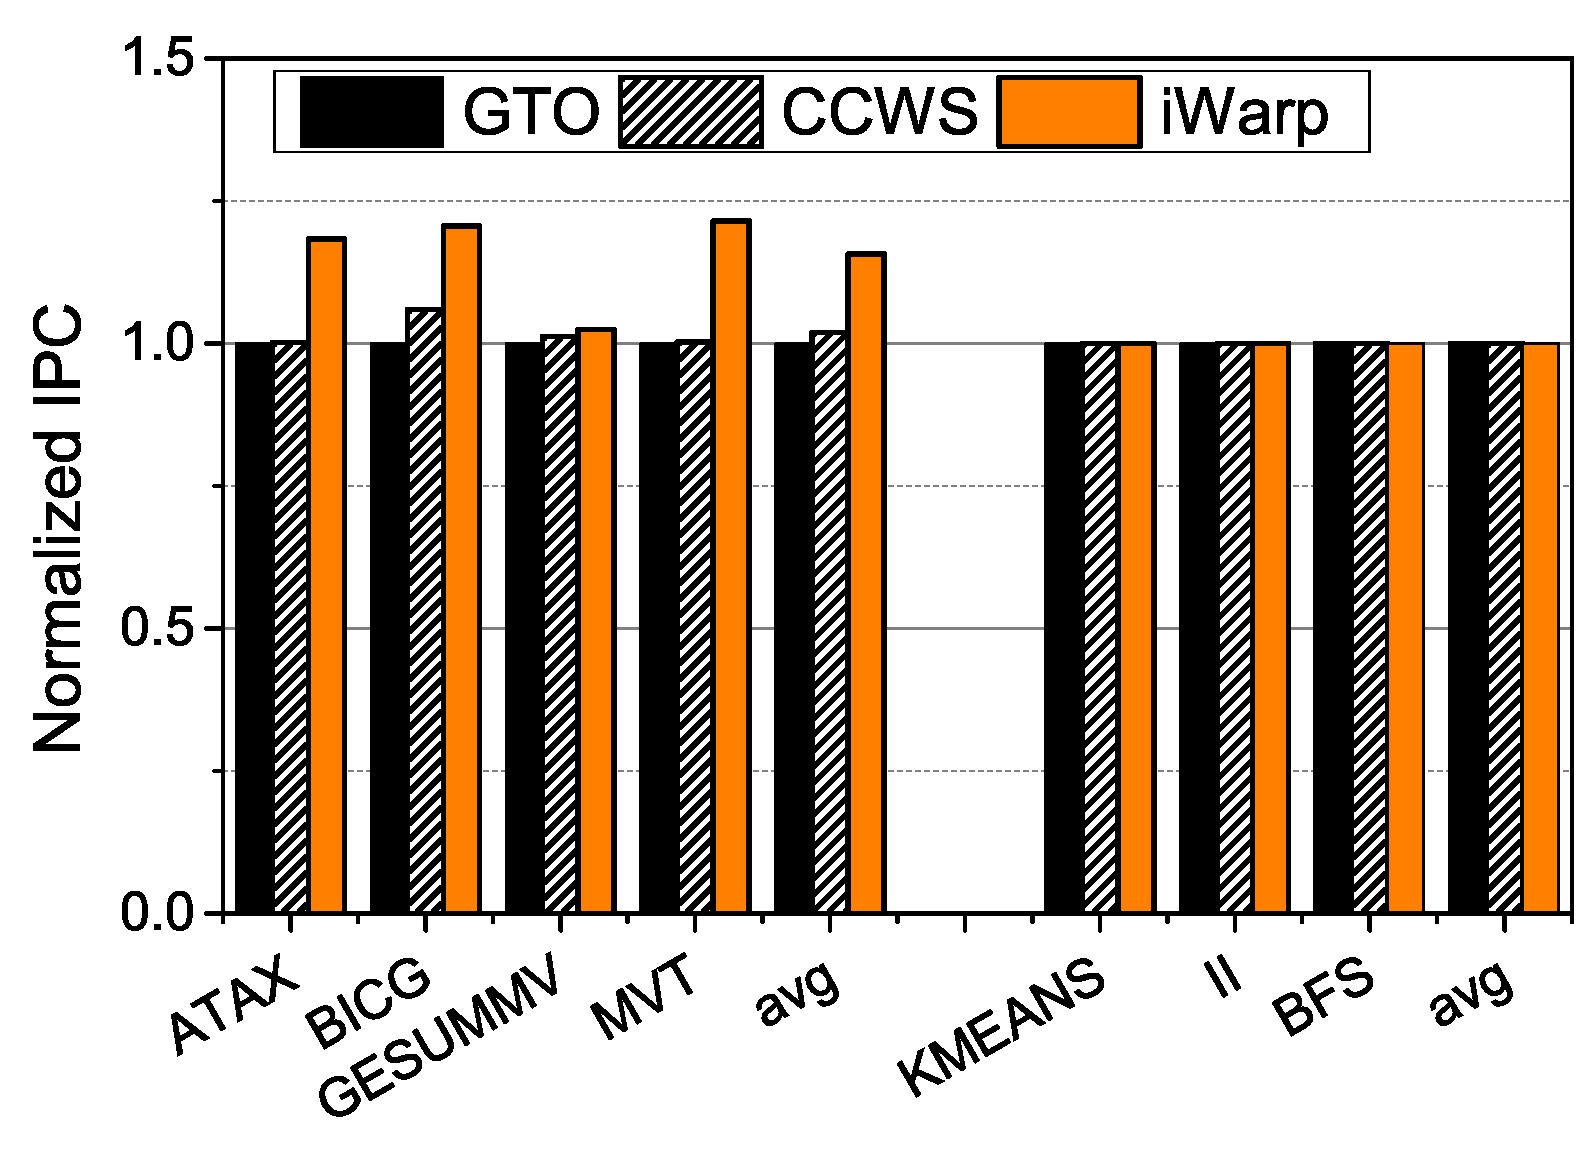
\epsfig{file=figs/64k_ipc.eps,angle=-0,width=1\textwidth,totalheight=5in,clip=}}}
    }
\end{center}
\vspace{-10pt}
\begin{center}
\caption{\textbf{Overall performance improvement of CCWS and iWarp with different size of L1D cache, normalized to GTO. With a small 16KB L1D cache, CCWS and iWarp improve the performance of heavy memory intensive benchmarks of 5.4\% and 18.3\% over GTO, respectively. With a larger 48KB L1D cache size, CCWS and iWarp improve the performance of heavy memory intensive benchmarks of 8.3\% and 17.8\% over GTO, respectively. As the cache size is enlarged to 64KB, the improvement of CCWS decreases to 1.9\%, while iWarp sill achieves 15.8\% improvement over GTO. As the L1D cache size becomes larger, cache interference of moderate cache sensitive benchmarks decreases significantly, and thus CCWS and iWrap tend to have similar performance with GTO.
\label{fig:ipc}}}
\end{center}
\vspace*{-15pt}
\end{figure*}

\noindent \textbf{IPC.} Figure \ref{fig:ipc}


\begin{figure*}
  \begin{center}
    \mbox{
      \subfigure[16KB. \label{fig:16k_l1_miss_rate}]{\scalebox{0.32}{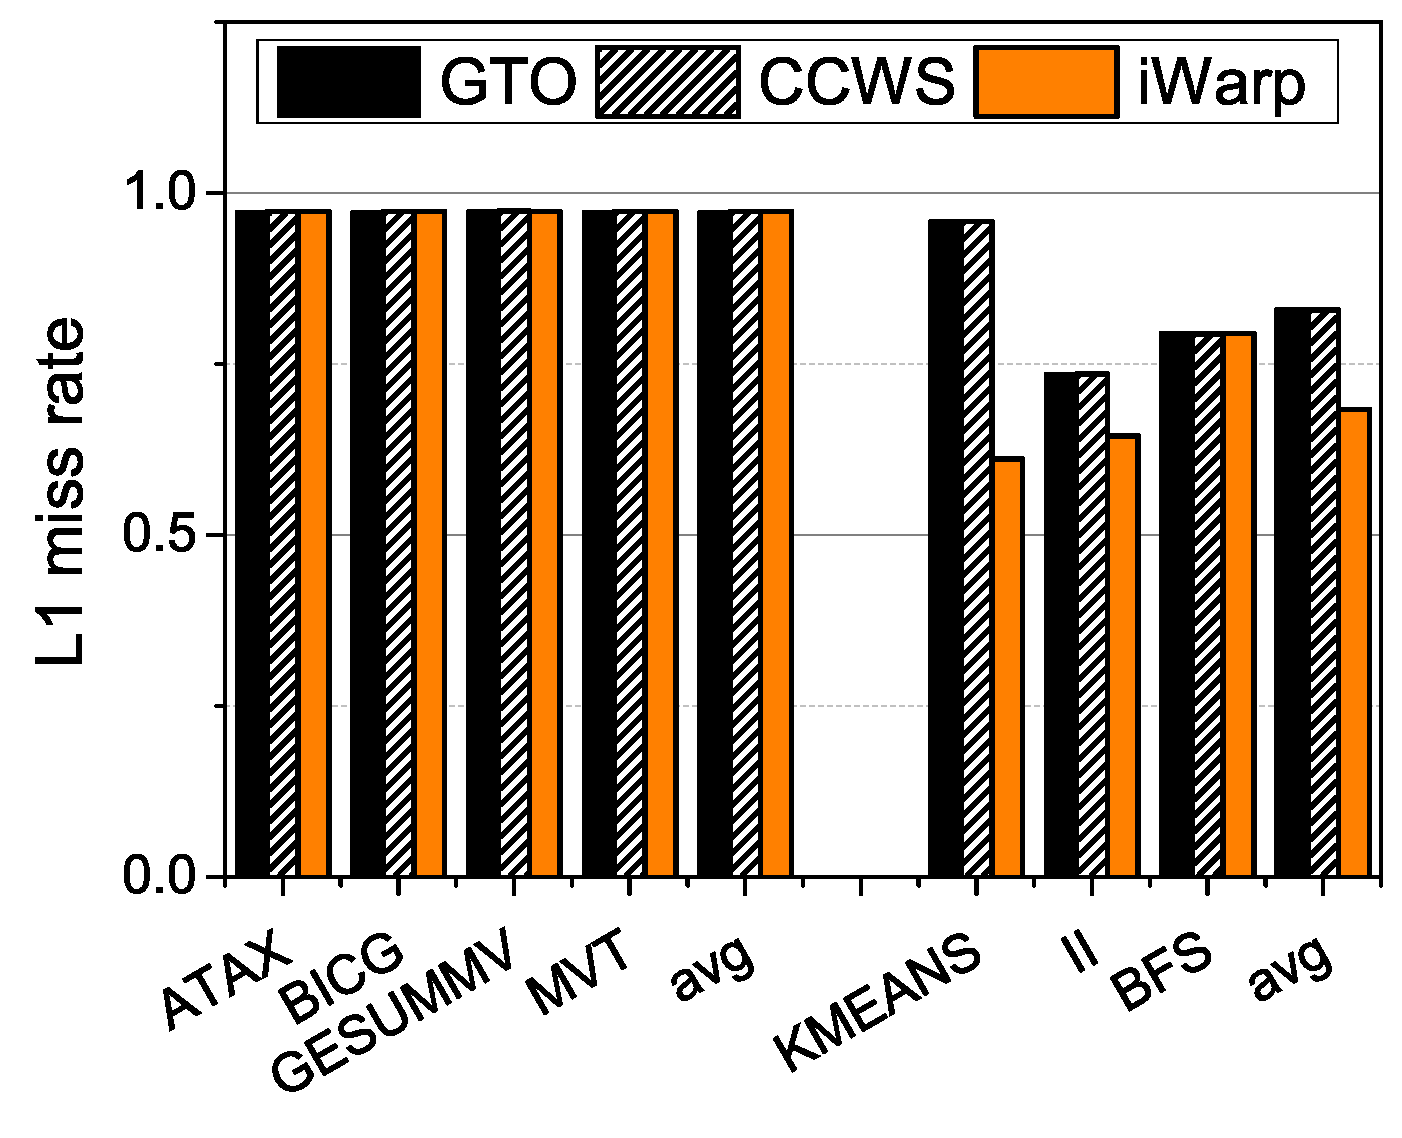
\epsfig{file=figs/16k_l1_miss_rate.eps,angle=-0,width=1\textwidth,totalheight=5in,clip=}}} \quad
      \subfigure[48KB. \label{fig:48k_l1_miss_rate}]{\scalebox{0.32}{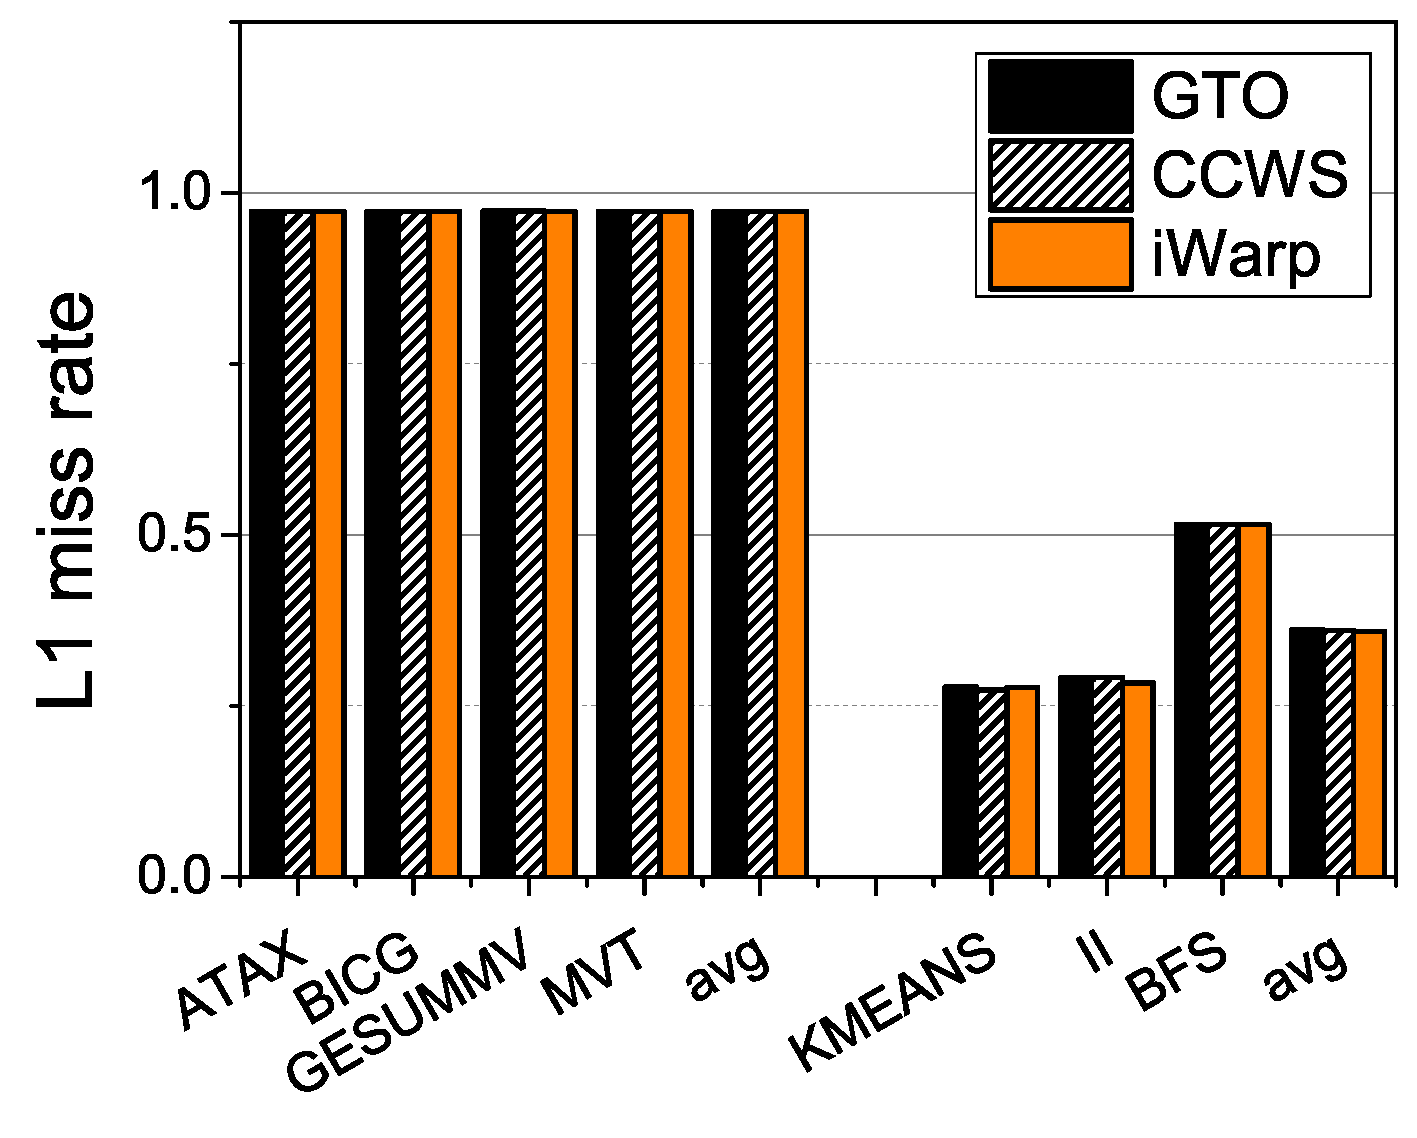
\epsfig{file=figs/48k_l1_miss_rate.eps,angle=-0,width=1\textwidth,totalheight=5in,clip=}}}\quad
      \subfigure[64KB. \label{fig:64k_l1_miss_rate}]{\scalebox{0.32}{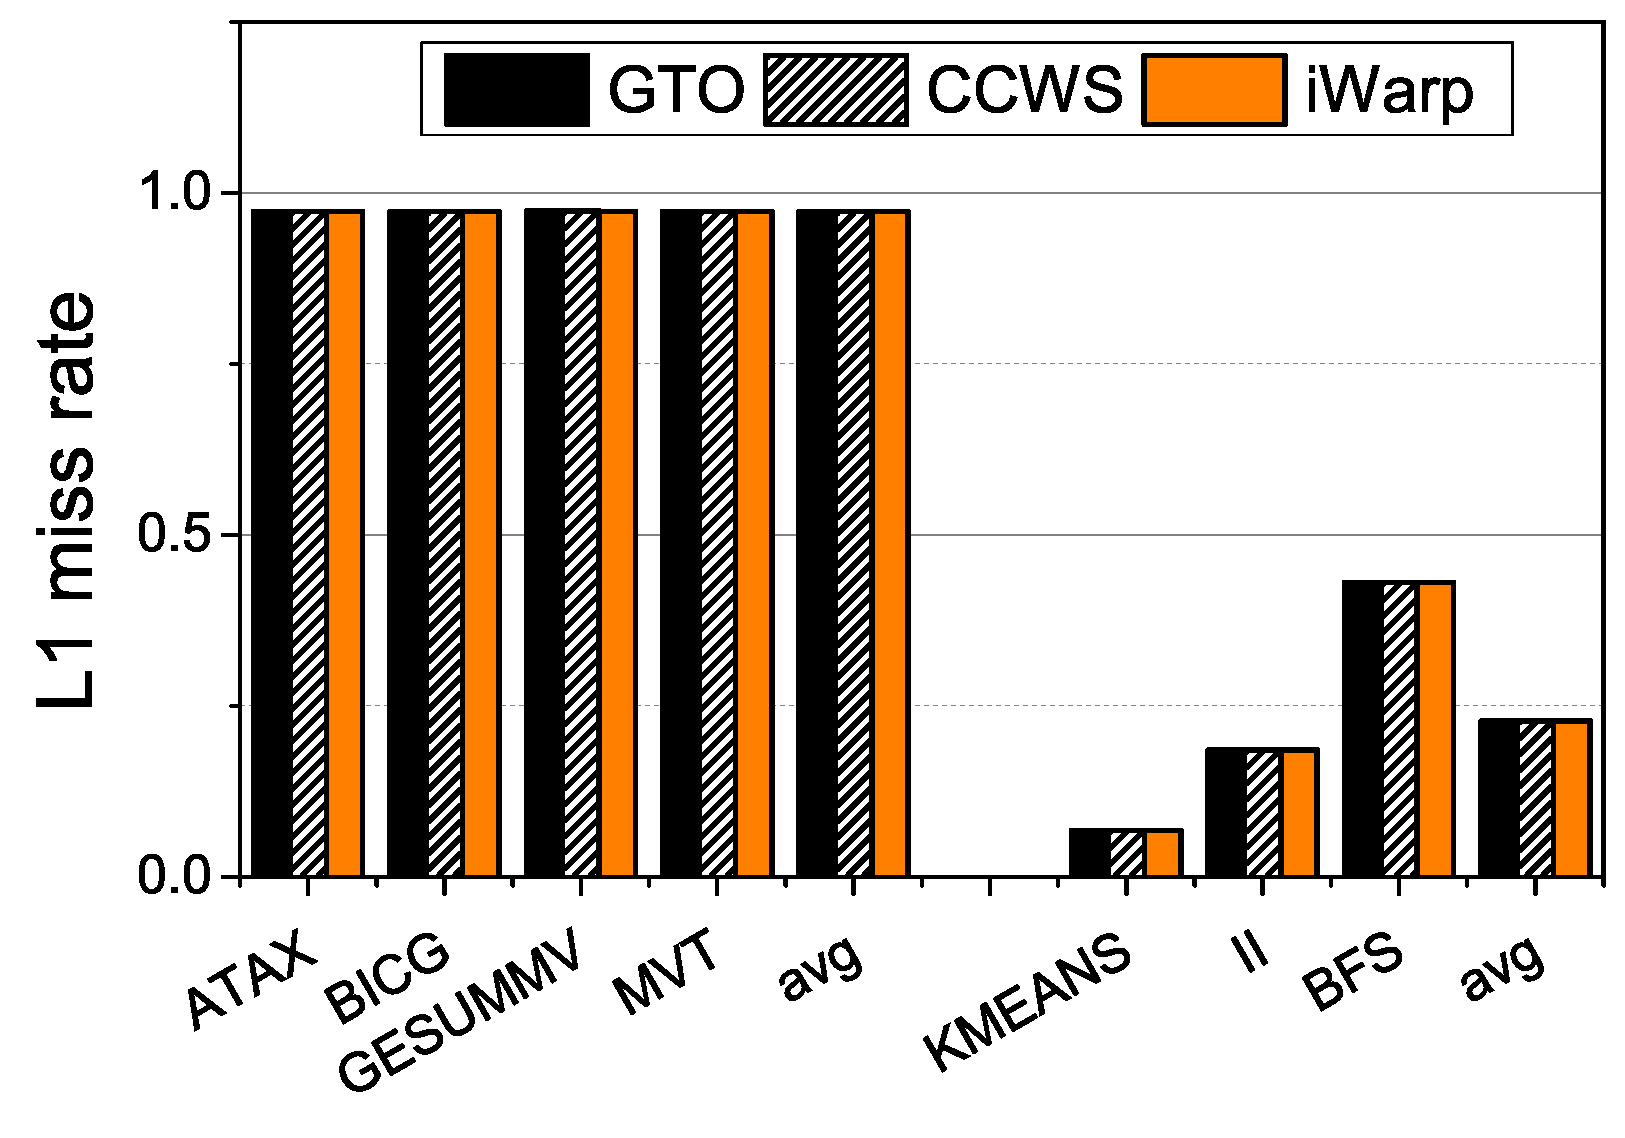
\epsfig{file=figs/64k_l1_miss_rate.eps,angle=-0,width=1\textwidth,totalheight=5in,clip=}}}
    }
\end{center}
\vspace{-10pt}
\begin{center}
\caption{\textbf{L1 miss rate of three schedulers. For heavy memory intensive benchmarks, the L1 miss rates with different warp schedulers are similar due to the huge intra-warp contention. For moderate memory intensive benchmarks, CCWS and iWrap reduces the L1 miss rate with small 16KB L1D cache, and have similar L1 miss rate with GTO with larger L1D cache. \label{fig:l1_miss_rate}}}
\end{center}
\vspace*{-15pt}
\end{figure*}

\begin{figure*}
  \begin{center}
    \mbox{
      \subfigure[16KB. \label{fig:16k_12_miss_rate}]{\scalebox{0.32}{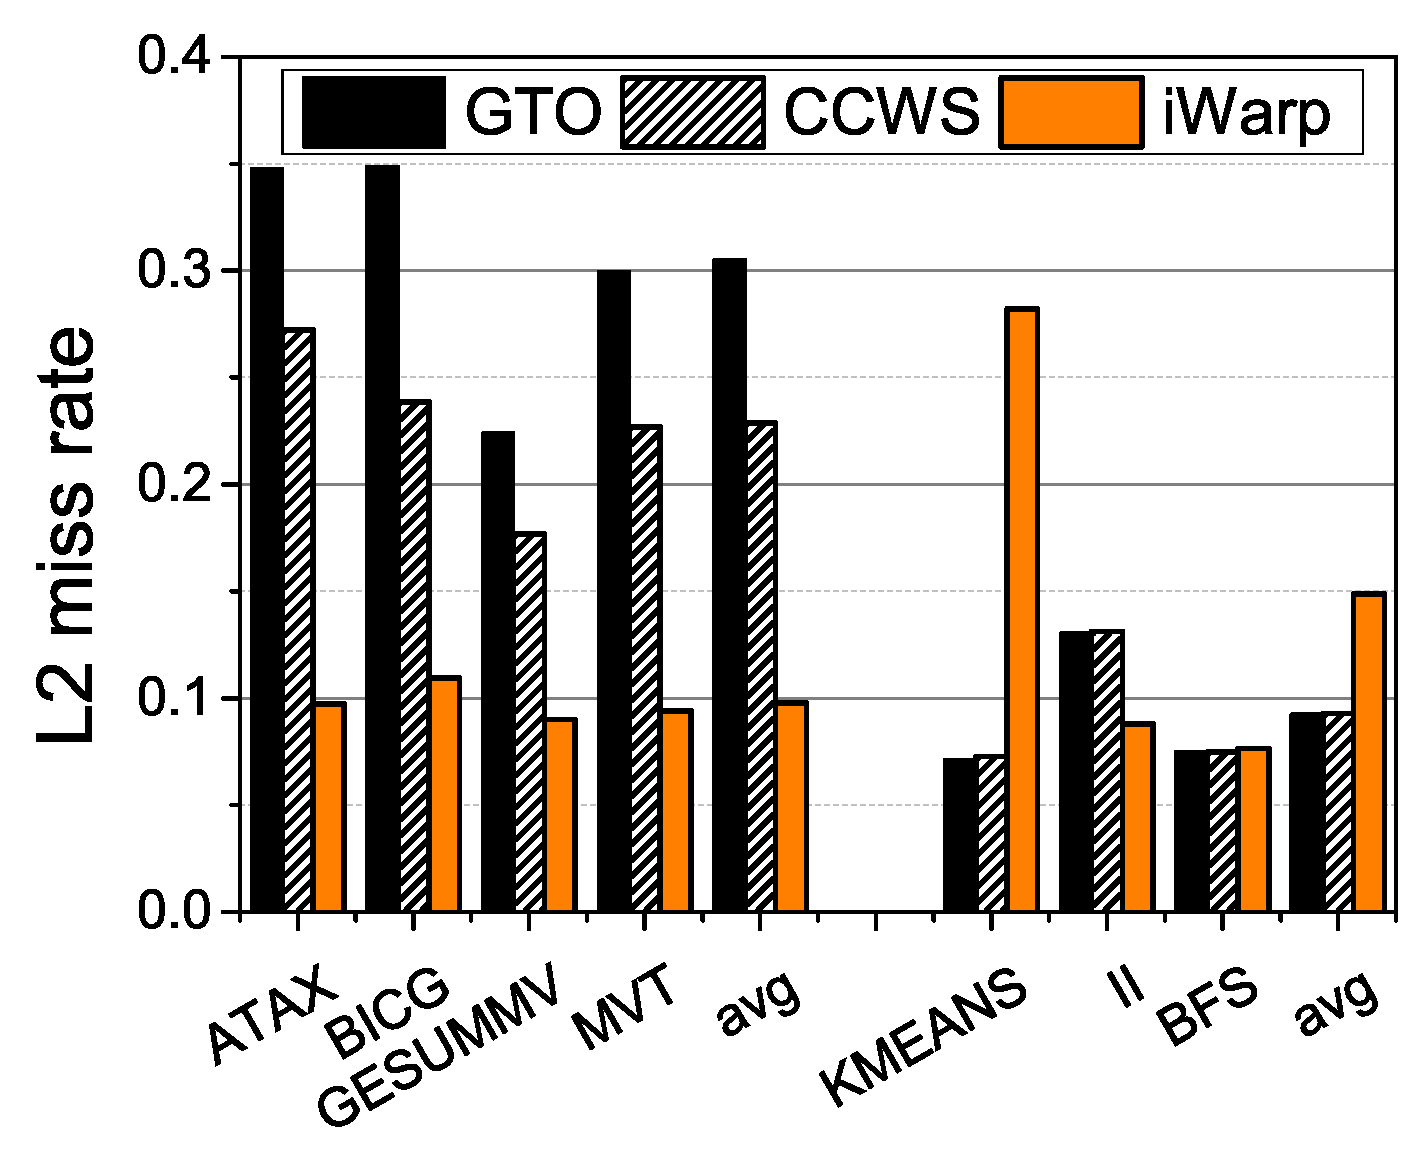
\epsfig{file=figs/16k_l2_miss_rate.eps,angle=-0,width=1\textwidth,totalheight=5in,clip=}}} \quad
      \subfigure[48KB. \label{fig:48k_l2_miss_rate}]{\scalebox{0.32}{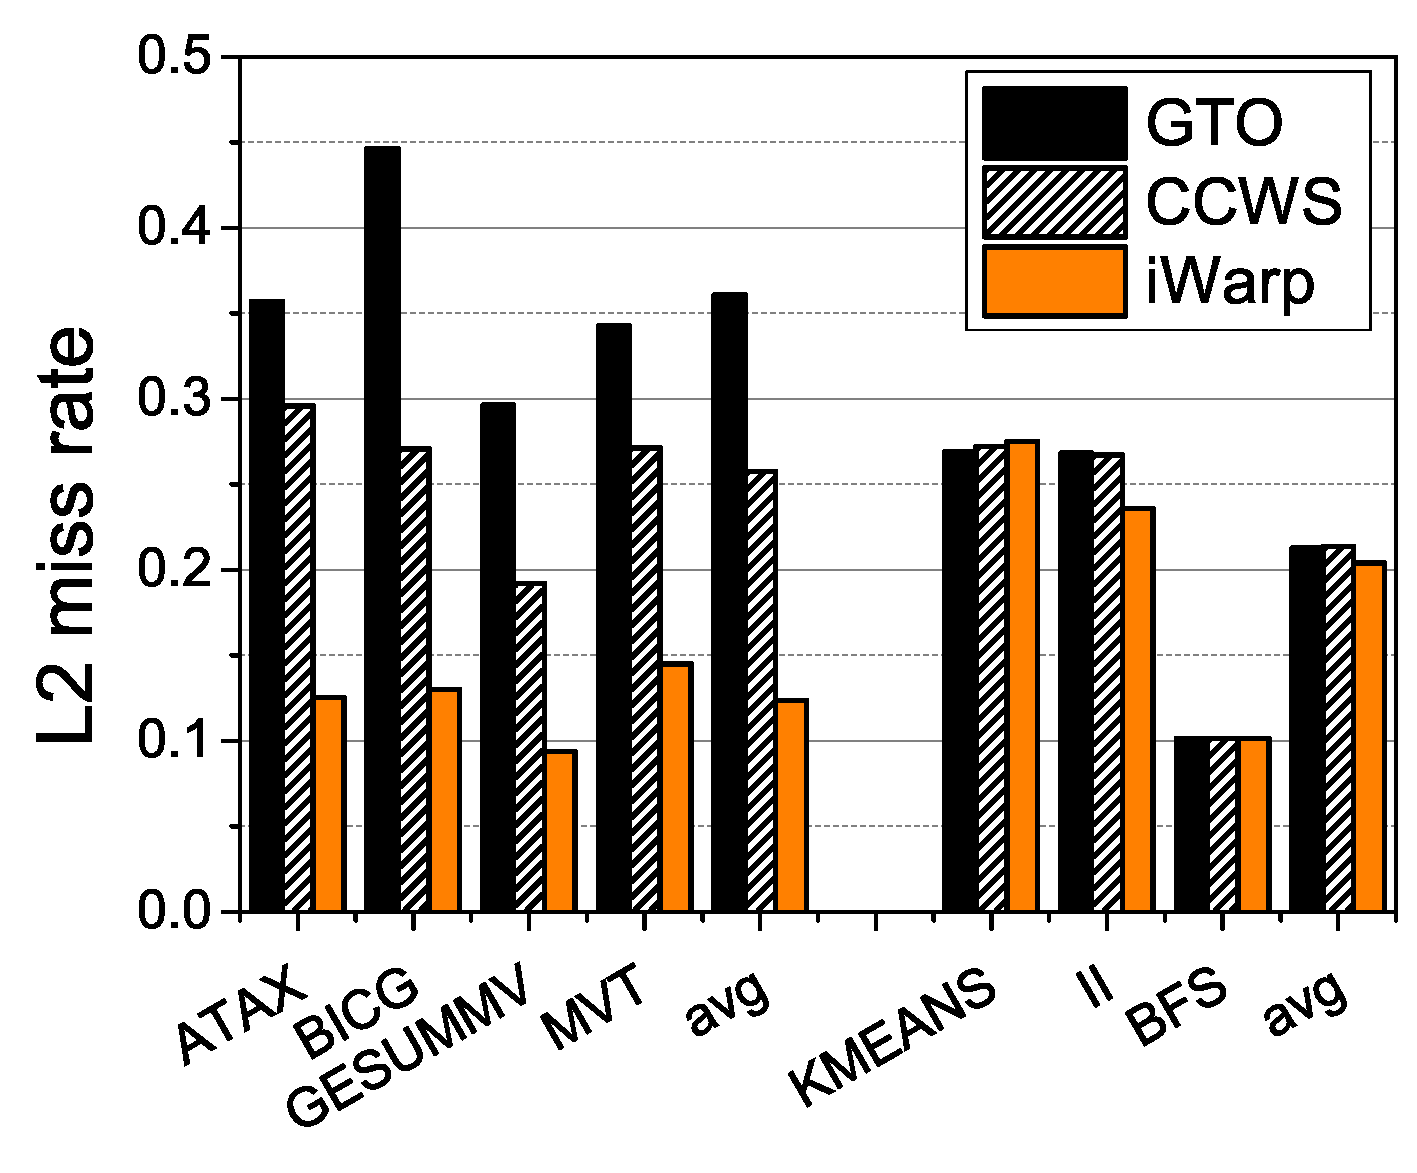
\epsfig{file=figs/48k_l2_miss_rate.eps,angle=-0,width=1\textwidth,totalheight=5in,clip=}}}\quad
      \subfigure[64KB. \label{fig:64k_l2_miss_rate}]{\scalebox{0.32}{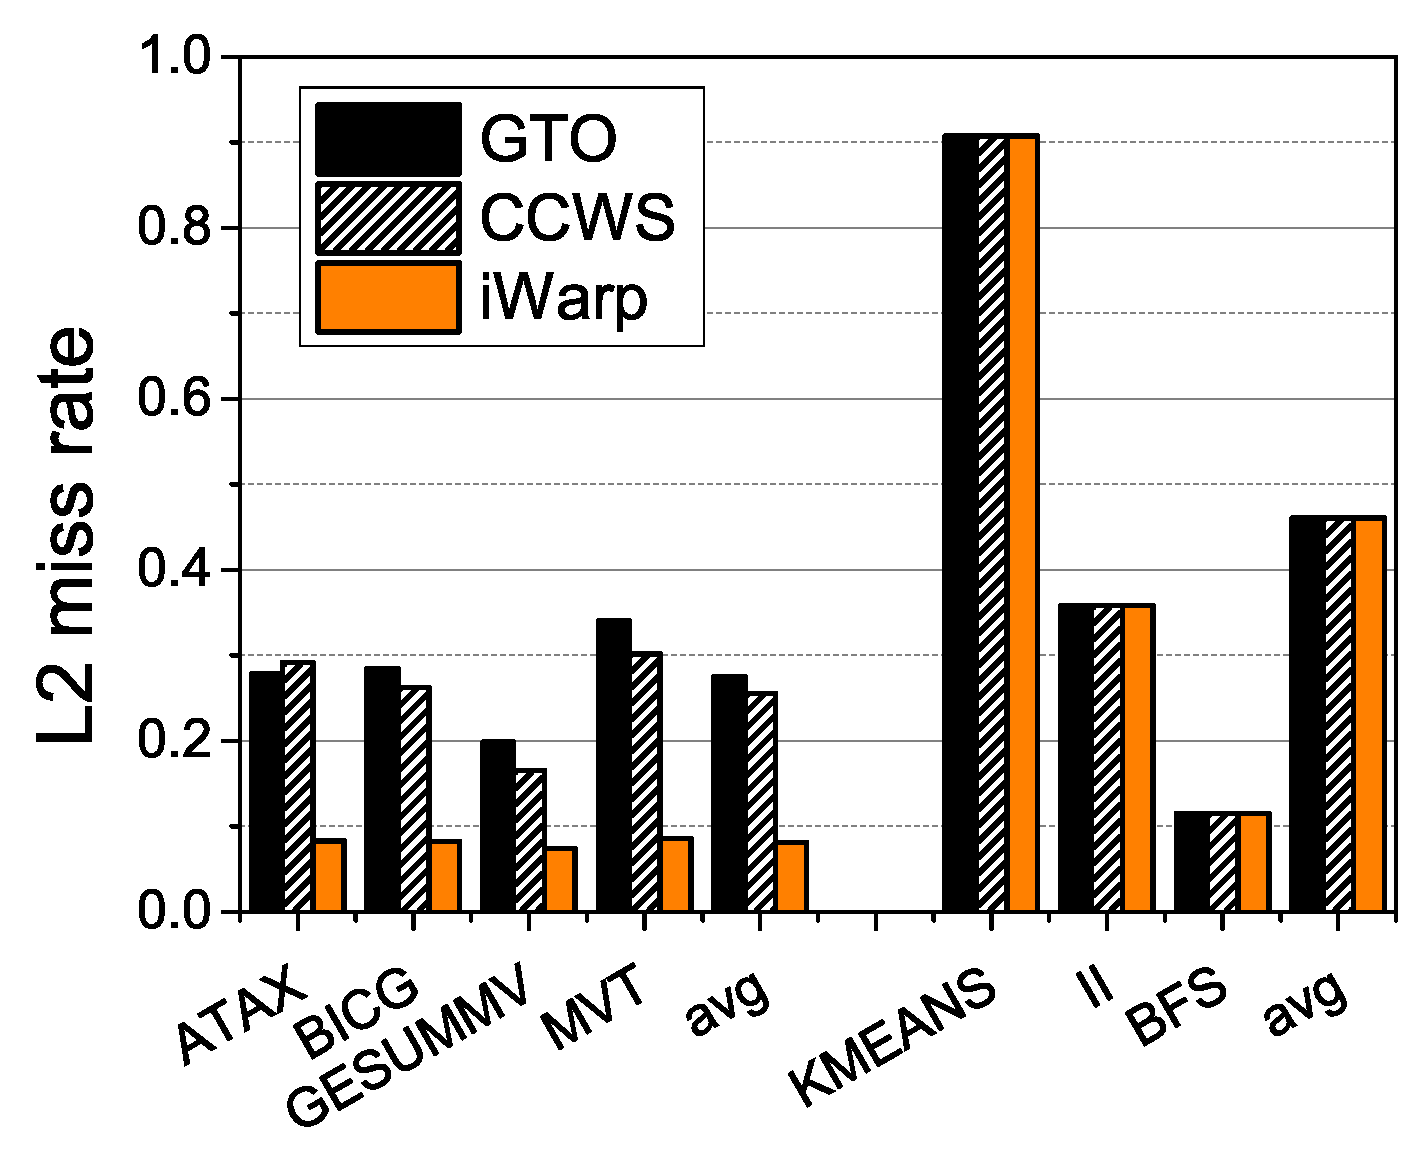
\epsfig{file=figs/64k_l2_miss_rate.eps,angle=-0,width=1\textwidth,totalheight=5in,clip=}}}
    }
\end{center}
\vspace{-10pt}
\begin{center}
\caption{\textbf{L2 miss rate of three schedulers. For heavy memory intensive benchmarks, iWarp achieves the lowest L2 miss rate among the three schedulers with different size of L1D cache.
\label{fig:l2_miss_rate}}}
\end{center}
\vspace*{-15pt}
\end{figure*}

\noindent \textbf{Cache Misses in L1 and L2.} Figure \ref{fig:l1_miss_rate} and Figure \ref{fig:l2_miss_rate}

\begin{figure*}
  \begin{center}
    \mbox{
      \subfigure[16KB. \label{fig:16k_avg_mf}]{\scalebox{0.32}{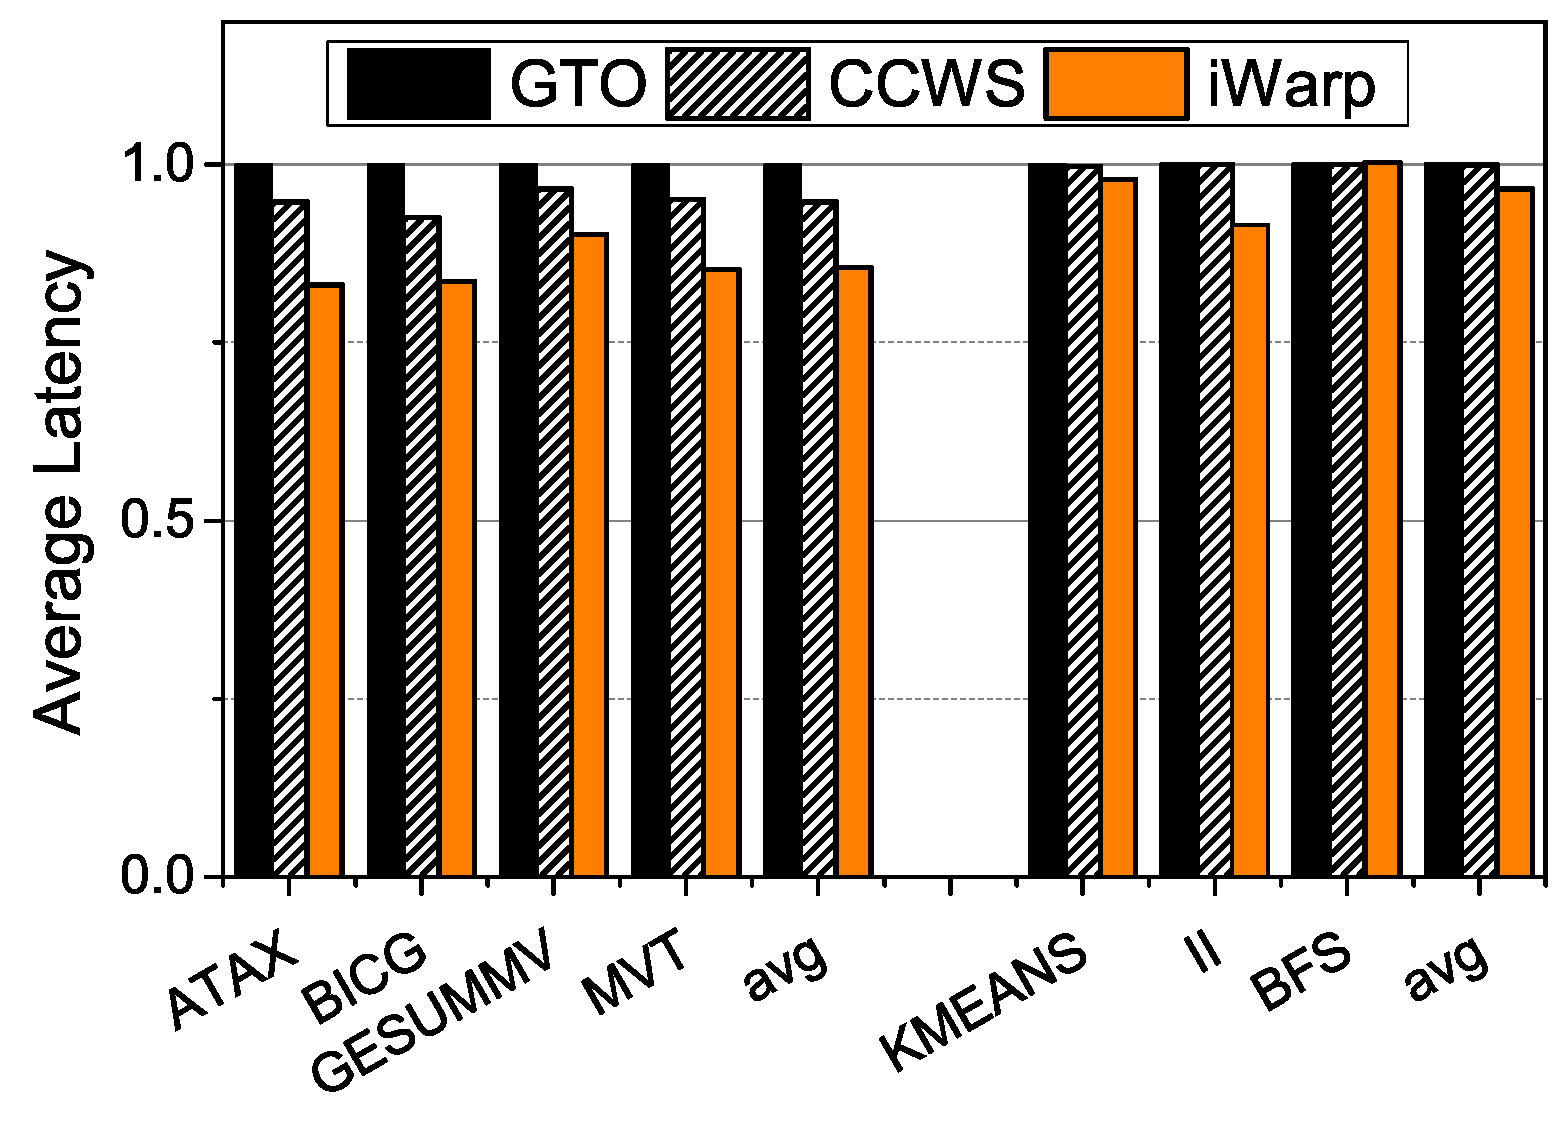
\epsfig{file=figs/16k_avg_mf.eps,angle=-0,width=1\textwidth,totalheight=5in,clip=}}} \quad
      \subfigure[48KB. \label{fig:48k_avg_mf}]{\scalebox{0.32}{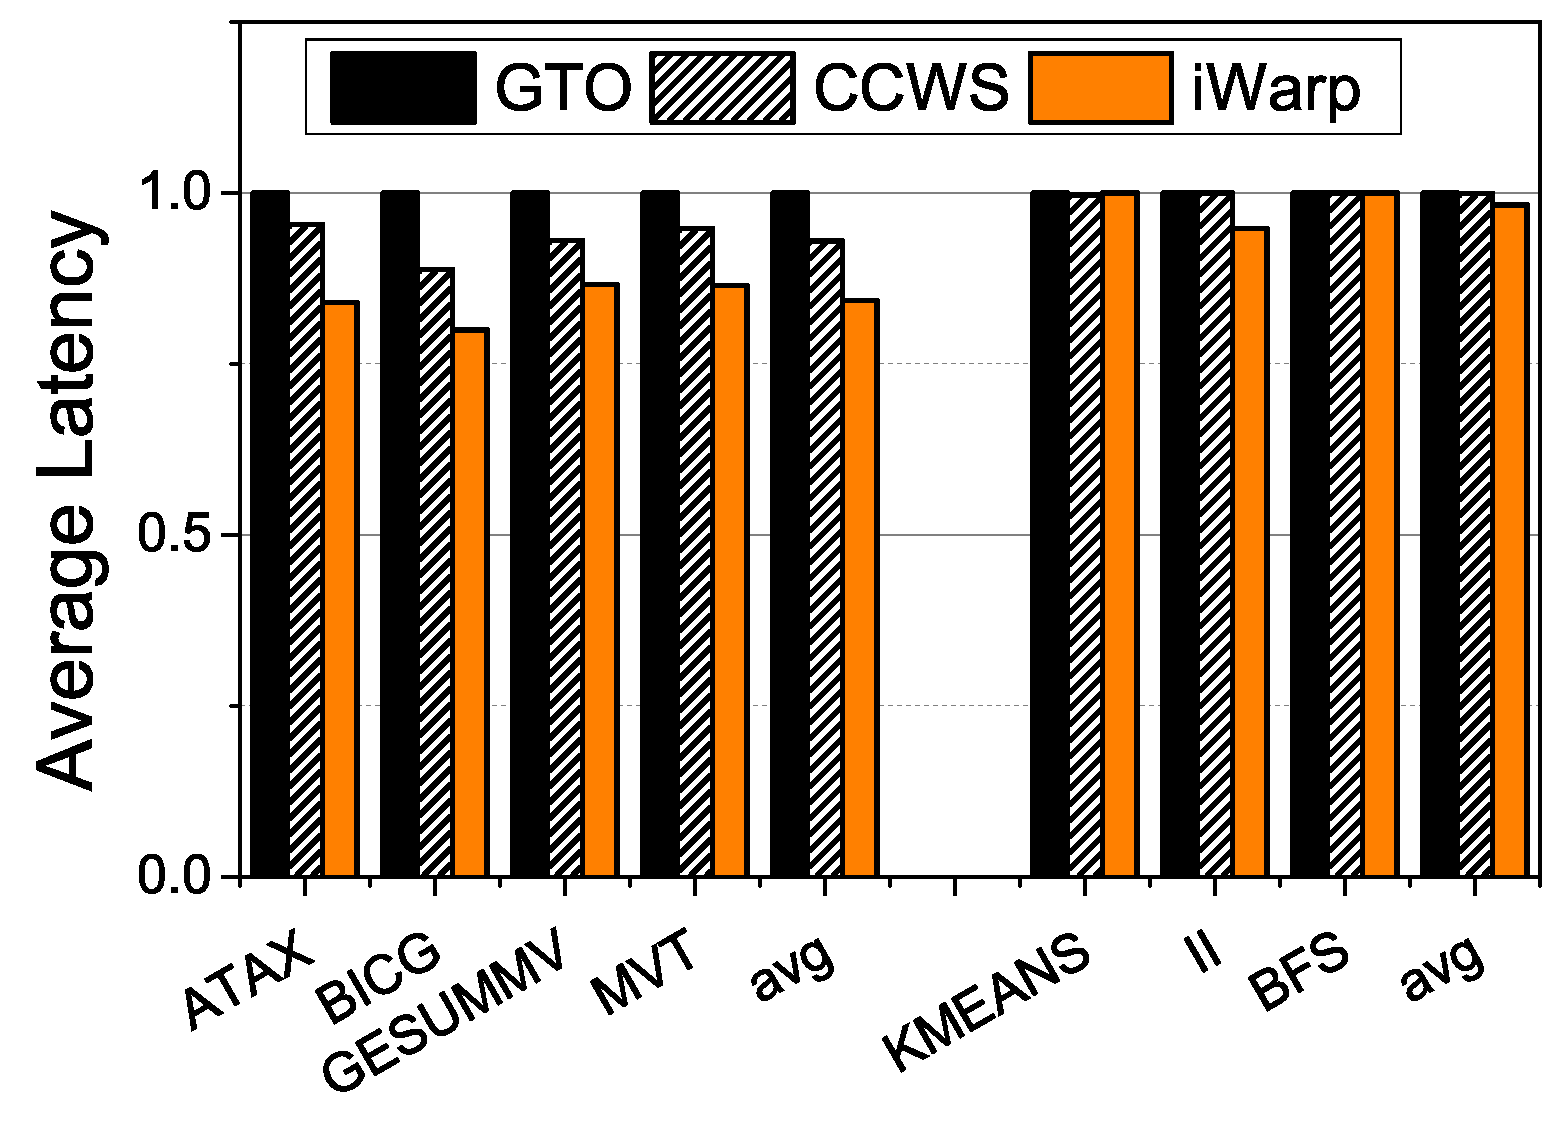
\epsfig{file=figs/48k_avg_mf.eps,angle=-0,width=1\textwidth,totalheight=5in,clip=}}}\quad
      \subfigure[64KB. \label{fig:64k_avg_mf}]{\scalebox{0.32}{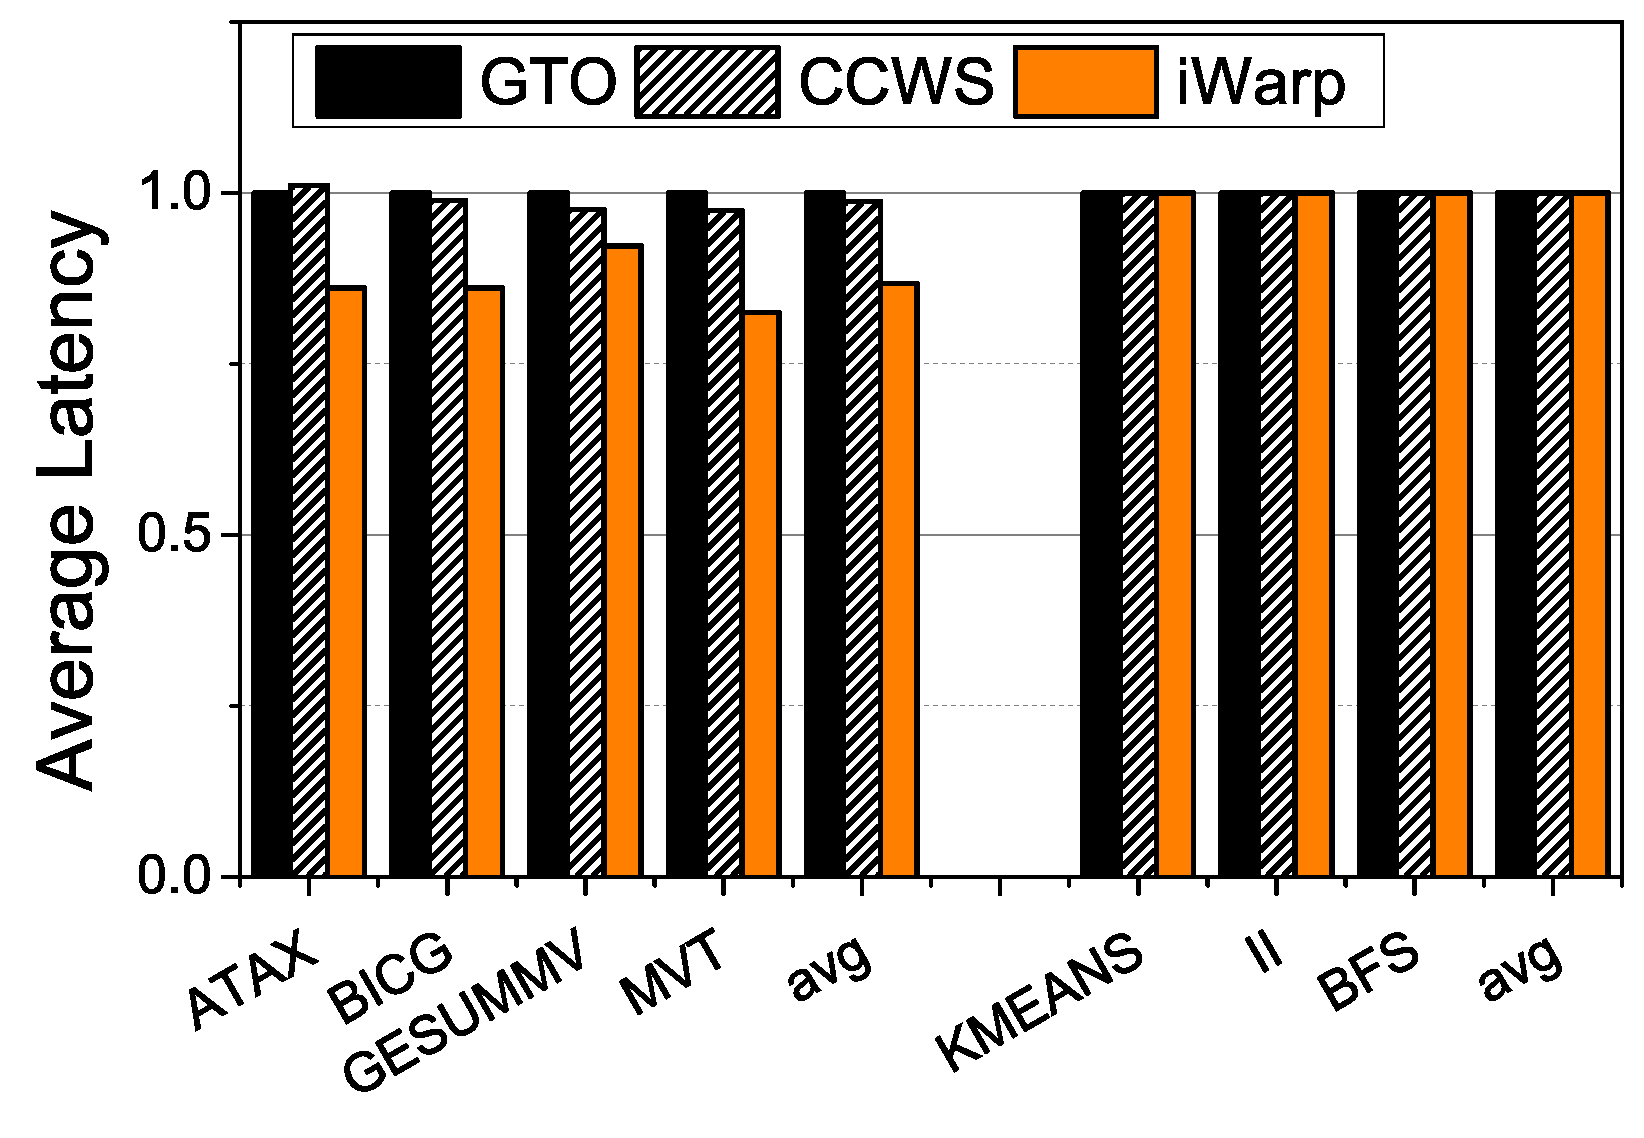
\epsfig{file=figs/64k_avg_mf.eps,angle=-0,width=1\textwidth,totalheight=5in,clip=}}}
    }
\end{center}
\vspace{-10pt}
\begin{center}
\caption{\textbf{Average memory fetch latency of three schedulers, normalized to GTO. For heavy memory intensive benchmarks, iWarp achieves the shortest average memory fetch latency among the three schedulers with different size of L1D cache. \label{fig:mf}}}
\end{center}
\vspace*{-15pt}
\end{figure*}

\noindent \textbf{DRAM accesses.} Figure \ref{fig:mf}

\appendix
\section{Appendix Title}

This is the text of the appendix, if you need one.

\acks

Acknowledgments, if needed.

% We recommend abbrvnat bibliography style.

%\bibliographystyle{abbrvnat}
%
%% The bibliography should be embedded for final submission.
%
%\begin{thebibliography}{}
%\softraggedright
%
%\bibitem[Smith et~al.(2009)Smith, Jones]{smith02}
%P. Q. Smith, and X. Y. Jones. ...reference text...
%
%\end{thebibliography}
\bibliographystyle{acm}
\bibliography{iWarp}

\end{document}

%                       Revision History
%                       -------- -------
%  Date         Person  Ver.    Change
%  ----         ------  ----    ------

%  2013.06.29   TU      0.1--4  comments on permission/copyright notices

